\documentclass[12pt]{article}

\usepackage{booktabs}% http://ctan.org/pkg/booktabs
\usepackage[utf8]{inputenc}
\usepackage{changepage}
\usepackage{pgfplots}
\usepackage{amssymb}
\usepackage{xcolor}
\usepackage{hyperref}
\usepackage{listings}
\usepackage[T1]{fontenc}
\usepackage[utf8]{inputenc}
\usepackage{adjustbox}
\usepackage{amsmath}
\usepackage{mathtools}
\usepackage{biblatex}
\lstset{
  language=Python,
  numbers=left,
  numberstyle=\tiny,
  stepnumber=1,
  numbersep=5pt,
  tabsize=4,
  basicstyle=\ttfamily,
  columns=fullflexible,
  keepspaces,
}
\hypersetup{
    colorlinks,
    citecolor=black,
    filecolor=black,
    linkcolor=black,
    urlcolor=black
}

% Set page size and margins
% Replace `letterpaper' with `a4paper' for UK/EU standard size
\usepackage[letterpaper,top=2cm,bottom=2cm,left=3cm,right=3cm,marginparwidth=1.75cm]{geometry}

% Useful packages
\usepackage{amsmath}
\usepackage{mathtools}
\usepackage{graphicx}
\newenvironment{para}{\begin{adjustwidth}{13mm}{}}{\end{adjustwidth}}

\newcommand\tab[1][1cm]{\hspace*{#1}}

\newcommand{\tabitem}{\llap{\textbullet}}
\newcommand{\Hsquare}{%
\text{\fboxsep=-.2pt\fbox{\rule{0pt}{1ex}\rule{1ex}{0pt}}}%
}

\newtheorem{Definizione}{Definizione}[subsection]
\newtheorem{Lemma}{Lemma}[subsection]
\newtheorem{Teorema/Definizione}{Teorema/Definizione}[subsection]
\newtheorem{Corollario}{Corollario}[subsection]
\newtheorem{Teorema}{Teorema}[subsection]
\newtheorem{Proposizione}{Proposizione}[subsection]
\newtheorem{Notazione}{Notazione}[subsection]
\newtheorem{Commento}{Commento}[subsection]
\newtheorem{Dimostrazione}{Dimostrazione}[subsection]
\newtheorem{Osservazione}{Osservazione}[subsection]
\newtheorem{Nota}{Nota}[subsection]

\title{Basi di dati}
\author{spitfire}
\date{A.A. 2023-2024}
\begin{document}
\begin{figure}
    \centering
    
\includegraphics[width=0.35\textwidth]{Images/Logo scienze bicocca.png}
\end{figure}

\vspace{10cm}
\date{A.A. 2023-2024}


\maketitle

\newpage

\tableofcontents
\newpage
\section{Introduzione}
Una base di dati è un \textbf{insieme organizzato di dati} utilizzati per il supporto allo svolgimento di attività (di un ente, azienda, ufficio, persona).
Facciamo un passo indietro e ricordiamo cos'è invece \textbf{l'informatica}:
essa è la \textbf{scienza del trattamento razionale dell'informazione}, spesso per mezzo di \textbf{macchine automatiche}.
Essa è considerata come supporto alla conoscenza umana e alla comunicazione.
L'informatica ha due anime:
\begin{itemize}
    \item \textbf{Metodologica}: i metodi per la soluzione di problemi e la gestione delle informazioni
    \item \textbf{Tecnologica}: i calcolatori elettronici e i sistemi che li utilizzano
\end{itemize}
\subsection{Sistemi informativi}
Un \textbf{sistema informativo} è un componente (sottosistema) di un'organizzazione che gestisce le informazioni di interesse (cioè utilizzate per il perseguimento degli scopi dell'organizzazione).
Le funzioni di un sistema informativo sono:
\begin{itemize}
    \item \textbf{Acquisizione/memorizzazione}
    \item \textbf{Aggiornamento}
    \item \textbf{Interrogazione}
    \item \textbf{Elaborazione}
\end{itemize}
Il concetto di "sistema informativo" è \textbf{indipendente da qualsiasi automazione}: esistono organizzazioni
la cui ragion d'essere è la \textbf{gestione di informazioni} (es. servizi anagrafici e banche) e che operano da secoli.
Anche prima di essere automatizzati, molti sistemi informativi si sono evoluti verso una \textbf{razionalizzazione e standardizzazione} delle procedure e dell'organizzazione delle informazioni.
\subsection{Sistema informatico}
Un \textbf{sistema informatico} è una porzione \textbf{automatizzata} di un sistema informativo; cioè la parte del sistema informativo che gestisce le informazioni con tecnologia informatica.
\begin{center}
    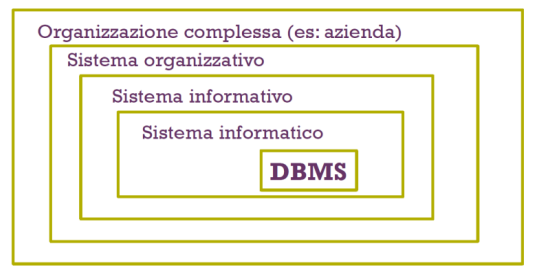
\includegraphics[width = 0.55\textwidth]{Images/1.PNG}
\end{center}
\newpage
\noindent
Un sistema informatico:
\begin{itemize}
    \item Garantisce che i dati siano conservati in modo \textbf{permanente} sui dispositivi di memorizzazione
    \item Permette un \textbf{rapido aggiornamento} dei dati per riflettere rapidamente le loro variazioni
    \item Rende i dati \textbf{accessibili alle interrogazioni} degli utenti
    \item Può essere \textbf{distribuito sul territorio}
\end{itemize}
\subsection{Gestione delle informazioni}
Nelle attività umane, le informazioni vengono gestite (registrate e scambiate) in forme diverse:
\begin{itemize}
    \item \textbf{Idee informali}
    \item \textbf{Linguaggio naturale} (scritto o parlato, formale o colloquiale, in una lingua o in un'altra)
    \item \textbf{Disegni, grafici e schemi}
    \item \textbf{Numeri e codici}
\end{itemize}
E su vari supporti, come la memoria umana, su carta o su dispositivi elettronici.
Nelle attività standardizzate dei sistemi informativi complessi, sono state introdotte col tempo forme di organizzazione e codifica delle informazioni via via più precise (e in un certo senso artificiali).
Ad esempio, nei servizi anagrafici si è iniziato con registrazioni discorsive per poi evolversi in registrazioni più complete.
\subsection{Informazioni e dati}
Nei sistemi informatici (e non solo), le \textbf{informazioni} vengono rappresentate in modo essenziale, spartano: attraverso i \textbf{dati}.
Diamo delle definizioni semantiche:
\begin{itemize}
    \item \textbf{Informazione}: notizia, dato o elemento che consente di avere conoscenza più o meno esatta di fatti, situazioni, modi di essere.
    \item \textbf{Dato}: ciò che è immediatamente presente alla conoscenza, prima di ogni elaborazione; (in informatica) elementi di informazione costituiti da simboli che debbono essere elaborati
\end{itemize}
I dati quindi hanno bisogno di essere interpretati!
\subsubsection{Perché i dati?}
La rappresentazione precisa di forme più ricche di informazione e conoscenza è difficile.
I dati costituiscono spesso una risorsa strategica, perché più stabili nel tempo di altri componenti (processi, tecnologie, ruoli, umani).
I dati rimangono gli stessi nella \textbf{migrazione} da un sistema al successivo.
\subsection{Basi di Dati e introduzione ai Database Management Systems (DBMS)}
Come già detto, una \textbf{base di dati} (DB) è una collezione di dati utilizzati per rappresentare le informazioni di interesse in un sistema informativo.
Un \textbf{Database Management System} (DBMS) è invece un \textbf{sistema software} capace di gestire collezioni di dati che siano \textit{grandi, condivise e persistenti}, assicurando la loro \textit{affidabilità e privatezza}.
Possiamo quindi dare due accezioni al termine \textbf{base di dati}:
\begin{itemize}
    \item \textbf{Metodologica}: insieme organizzato di dati utilizzati per il supporto allo svolgimento delle attività di un ente
    \item \textbf{Specifica, metodologica e tecnologica}: Insieme di dati gestito da un DBMS
\end{itemize}
Possiamo dare ancora una definizione: una \textbf{base di dati} è un insieme di archivi in cui ogni dato è rappresentato logicamente
una sola volta e può essere utilizzato da un insieme di applicazioni o da diversi utenti secondo opportuni criteri di riservatezza.
\begin{center}
    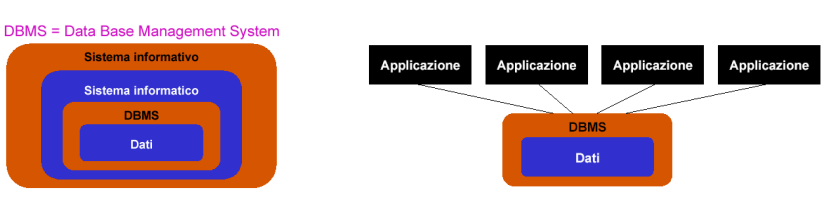
\includegraphics[width = 1\textwidth]{Images/2.PNG}
\end{center}
Le caratteristiche di una base di dati sono:
\begin{itemize}
    \item I dati sono \textbf{molti}
    \item I dati hanno un \textbf{formato definito}
    \item I dati sono \textbf{permanenti}
    \item I dati sono \textbf{raggruppati} per insiemi \textbf{omogenei} di dati
    \item Esistono \textbf{relazioni specifiche} tra gli insiemi di dati
    \item La ridondanza è \textbf{minima e controllata}: è assicurata la consistenza delle informazioni
    \item I dati sono disponibili \textbf{per utenze diverse e concorrenti}
    \item I dati sono \textbf{controllati}: protetti da malfunzionamenti hardware e software
    \item I dati della base di dati sono \textbf{indipendenti dai dati di un qualsiasi programma}
\end{itemize}
\subsection{Database Management System}
Un DBMS è un insieme di programmi che permettono di creare, usare e gestire una base di dati.
Quindi un DBMS è un sistema software general purpose che facilita il processo di \textbf{definizione, costruzione e manipolazione} del database per varie applicazioni.
Vi sono 3 fasi nella \textbf{creazione di un database}:
\begin{enumerate}
    \item \textbf{Definizione}
    \item \textbf{Creazione/Popolazione}
    \item \textbf{Manipolazione}
\end{enumerate}
Una volta creato un database, si potranno effettuare su di esso delle \textbf{interrogazioni} (queries).
L'efficacia delle queries dipende da:
\begin{itemize}
    \item Conoscenza dle contenuto del DB
    \item Esperienza con il linguaggio di interrogazione
    \item Semplicità ed efficacia dell'interfaccia di interrogazione
\end{itemize}
Un DBMS è quindi un \textbf{sistema} che gestisce collezioni di dati:
\begin{itemize}
    \item \textbf{Grandi}
    \item \textbf{Persistenti}
    \item \textbf{Condivise}
\end{itemize}
garantendo:
\begin{itemize}
    \item \textbf{Privatezza}
    \item \textbf{Affidabilità}
    \item \textbf{Efficienza}
    \item \textbf{Efficacia}
\end{itemize}
\subsection{Caratteristiche delle basi di dati}
Le basi di dato sono:
\begin{itemize}
    \item \textbf{Grandi}: dimensioni (molto) maggiori della memoria centrale dei sistemi di calcolo utilizzati. Il limite deve essere solo quello fisico dei dispositivi
    \item \textbf{Persistenti}: hanno un tempo di vita indipendente dalle singole esecuzioni dei programmi che le utilizzano
    \item \textbf{Condivise}: Ogni organizzazione (specie se grande) è divisa in settori o comunque svolge diverse attività. Ciascun settore/attività ha un (sotto)sistema informativo (non necessariamente disgiunto)
    \item I possibili problemi sono la \textbf{ridondanza}, cioè la ripetizione di informazioni, e \textbf{l'incoerenza}, cioè le varie versioni della basi di dati potrebbero non coincidere
\end{itemize}
\subsection{Archivi e basi di dati}
\begin{center}
    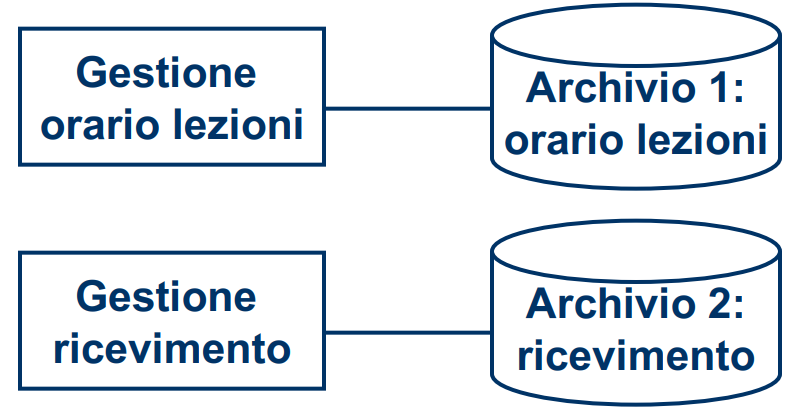
\includegraphics[width = 0.55\textwidth]{Images/3.PNG}
\end{center}
\begin{center}
    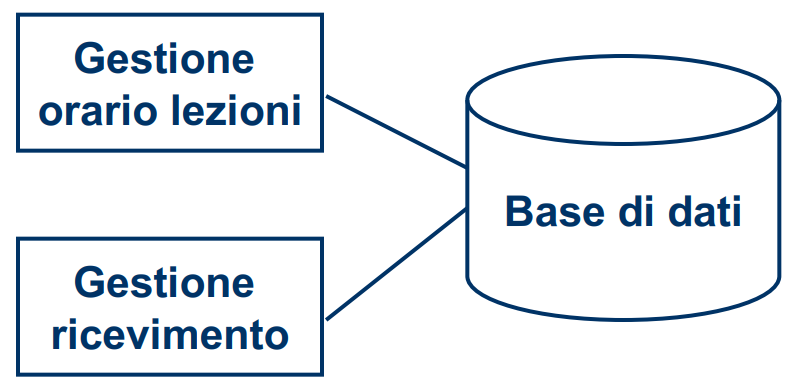
\includegraphics[width = 0.55\textwidth]{Images/4.PNG}
\end{center}
\subsection{Condivisione delle basi di dati}
Una base di dati è una risorsa \textbf{integrata e condivisa} fra applicazioni.
Diventa quindi possibile svolgere attività diverse su dati condivisi: sono necessari quindi \textbf{meccanismi di autorizzazione}.
Diventano anche possibili accessi di più utenti ai dati condivisi: sono quindi necessarie politiche e meccanismi di controllo della \textbf{concorrenza}.
\subsection{Caratteristiche dei DBMS}
I DBMS garantiscono \textbf{privatezza}; cioè si possono definire meccanismi di autorizzazione: l'utente A è, per esempio, autorizzato a leggere tutti i dati e a modificare quelli sul ricevimento; tuttavia
l'utente B è magari autorizzato a leggere i dati di X e a modificare i dati di Y. \newline
I DBMS garantiscono inoltre \textbf{l'affidabilità} dei dati, cioè la resistenza a malfunzionamenti hardware e software.
Per implementare questa caratteristica è quindi fondamentale \textbf{gestire le transazioni}.
\subsection{Transazioni}
Le \textbf{transazioni} sono l'insieme di operazioni da considerare indivisibili ("\textbf{atomiche}"), corrette anche in presenza di \textbf{concorrenza} e con effetti \textbf{definitivi}.
La sequenza di operazioni sulla base di dati viene eseguita per intero o per niente: per esempio, il trasferimento di fondi da un conto A ad un conto B avviene o tramite il prelevamento da A e il versamento su B o niente affatto.
L'effetto di transazioni concorrenti deve essere \textbf{coerente} (ad esempio "equivalente" all'esecuzione separata delle richieste concorrenti): per esempio, se due assegni emessi sullo stesso conto corrente vengono incassati \textbf{contemporaneamente},
si deve evitare di trascurarne uno.
La conclusione positiva di una transazione corrisponde ad un impegno (in inglese \textbf{commit}) a mantenere traccia del risultato in modo definitivo, anche in presenza di guasti e di esecuzione concorrente.
\subsection{Caratteristiche dei DBMS}
I DBMS devono essere \textbf{efficienti}, cioè devono cercare di utilizzare al meglio le risorse di spazio di memoria (principale e secondaria) e di tempo (di esecuzione e di risposta).
I DBMS, con tante funzioni, rischiano l'inefficienza e per questo ci sono grandi investimenti e competizione. L'efficienza è anche il risultato della qualità delle applicazioni. \newline
I DBMS devono essere \textbf{efficaci}, cioè devono cercare di rendere produttive le attività dei loro utilizzatori, offrendo funzionalità articolare, potenti e flessibili.
\subsection{Descrizioni dei dati nei DBMS}
Descrizioni e rappresentazione dei dati a livelli diversi permettono \textbf{l'indipendenza dei dati} dalla rappresentazione fisica: i programmi fanno riferimento alla struttura a livello più altro, e le rappresentazione sottostanti possono essere modificate senza necessità di modificare i programmi.
Possiamo precisare questo concetto attraverso il concetto di \textbf{modello dei dati}
\subsubsection{Modello dei dati}
Il \textbf{modello dei dati} è l'insieme di costrutti utilizzati per organizzare i dati di interesse e descriverne la dinamica.
Esso ha una componente fondamentale: i \textbf{meccanismi di strutturazione} (o \textbf{costruttori di tipo}): come nei linguaggi di programmazione
esistono meccanismi che permettono di definire nuovi tipi, così ogni modello dei dati prevede alcuni costruttori.
Ad esempio, il \textbf{modello relazionale} prevede il costruttore \textbf{relazione}, che permette di definire insiemi di record omogenei.
\subsection{Schema e istanza della base di dati}
\begin{center}
    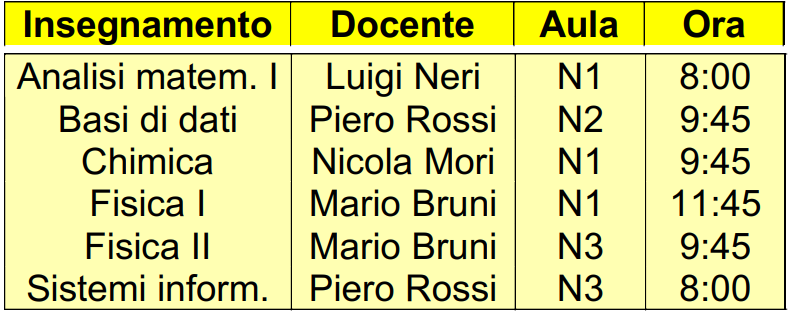
\includegraphics[width = 0.60\textwidth]{Images/5.PNG}
\end{center}
In ogni base di dati esistono:
\begin{itemize}
    \item Lo \textbf{schema}, sostanzialmente invariante nel tempo, che ne descriva la struttura e il significato (aspetto intensionale; es. le intestazioni delle tabelle). Lo schema quindi costituisce l'aspetto \textbf{intensionale}, ovvero la descrizione "astratta" delle proprietà, ed è invariante nel tempo
    \item \textbf{L'istanza}, i valori attuali, che possono cambiare anche molto rapidamente (aspetto estensionale; es. il "corpo" di ciascuna tabella). L'istanza quindi costituisce invece l'aspetto \textbf{estensionale} "concreto", che varia nel tempo al variare della situazione di ciò che stiamo descrivendo
\end{itemize}
\subsection{Modello dei dati logico}
I modelli dei dati logici sono adottati nei DBMS esistenti per l'organizzazione dei dati:
\begin{itemize}
    \item utilizzati dai programmi
    \item indipendenti dalle strutture fisiche
\end{itemize}
Esempi di essi sono il modello \textbf{relazionale}, reticolare, gerarchico, a oggetti, XML, ...
\subsubsection{Modello relazionale}
Nel modello relazionale i dati vengono strutturati in tabelle, in particolare un DBMS relazionale può essere pensato come un insieme di tabelle.
Ogni tabella mantiene informazioni di tipo omogeneo. Diverse tabelle sono collegate (in relazione) fra loro grazie alla presenza di un \textbf{campo comune}, che permette di mettere in relazione i dati delle due tabelle.
Nel modello relazionale:
\begin{itemize}
    \item \textbf{Lo schema} è la descrizione della struttura delle tabelle (stabile nel tempo)
    \item \textbf{L'istanza} sono i valori dei campi della tabella
\end{itemize}
\begin{center}
    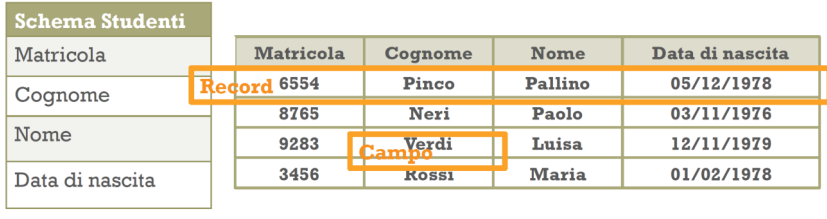
\includegraphics[width = 0.85\textwidth]{Images/6.PNG}
\end{center}
\subsection{Modello dei dati concettuale}
I modelli dei dati concettuali permettono di rappresentare i dati in modo indipendente da ogni sistema.
\begin{itemize}
    \item cercando di descrivere i concetti del mondo reale
    \item sono utilizzati nelle fasi preliminare di progettazione (quali informazioni sono utili? Come sono collegate?)
\end{itemize}
Il più diffuso è il modello \textbf{Entity-Relationship}
\newpage
\subsection{Architettura di un DBMS}
Possiamo strutturare l'architettura di un DBMS in maniera \textbf{semplificata} nel seguente modo:
\begin{center}
    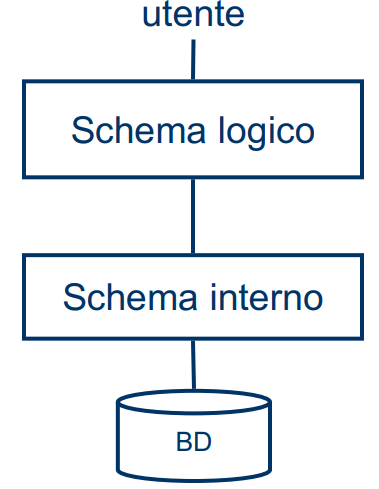
\includegraphics[width = 0.35\textwidth]{Images/7.PNG}
\end{center}
Nella quale:
\begin{itemize}
    \item \textbf{Schema logico}: descrizione della base di dati nel modello logico (ad esempio, la struttura della tabella)
    \item \textbf{Schema interno (o fisico)}: rappresentazione dello schema logico per mezzo di strutture di memorizzazione (file ad esempio, ma anche record con puntatori, ordinati in un certo modo)
\end{itemize}
Una delle architetture standard di riferimento per i DBMS è \textbf{L'architettura \newline ANSI/SPARC a tre livelli}:
\begin{center}
    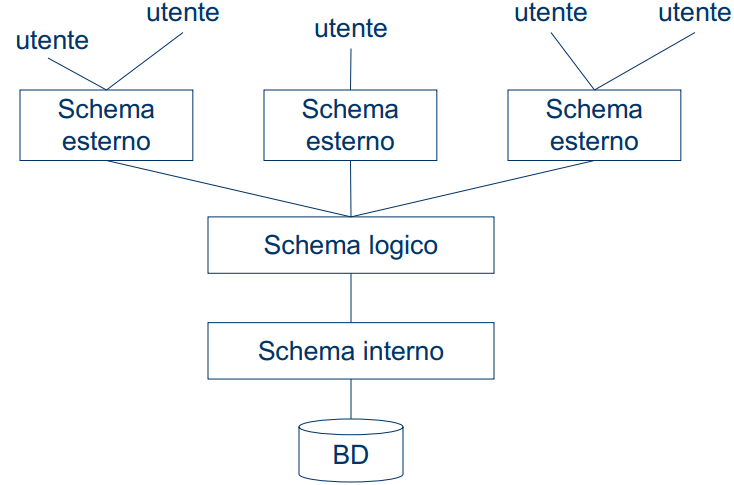
\includegraphics[width = 0.65\textwidth]{Images/8.PNG}
\end{center}
Nella quale:
\begin{itemize}
    \item \textbf{Schema logico}; descrizione dell'intera base di dati nel modello logico "principale" del DBMS
    \item \textbf{Schema fisico}: rappresentazione dello schema logico per mezzo di strutture fisiche di memorizzazione
    \item \textbf{Schema esterno}: descrizione di parte della base di dati in un modello logico ("viste" parziali, derivate, anche in modelli diversi)
\end{itemize}
\begin{center}
    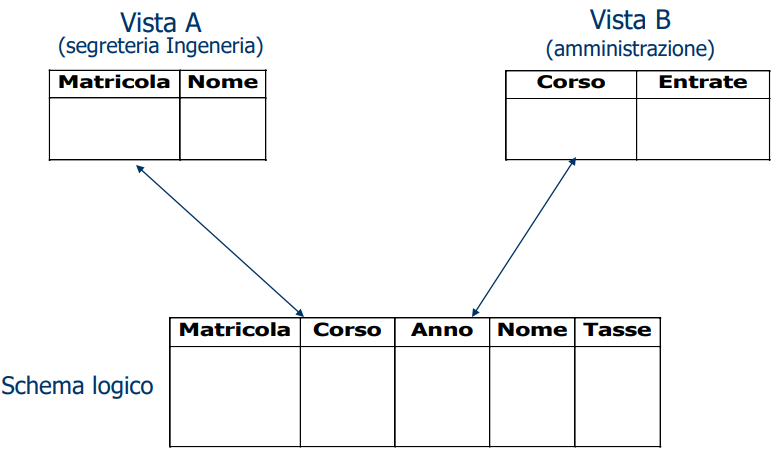
\includegraphics[width = 0.75\textwidth]{Images/9.PNG}
\end{center}
\subsection{Indipendenza dei dati}
Il livello logico è indipendente da quello fisico: una tabella è utilizzata nello stesso modo qualunque sia la sua realizzazione fisica (che può anche cambiare nel tempo).
In questo corso vedremo solo il livello logico e non quello fisico.
La conseguenza della articolazioni in livelli è che l'accesso avviene solo tramite il \textbf{livello esterno} (che può coincidere con il livello logico).
Vi sono due forme di indipendenza:
\begin{itemize}
    \item \textbf{Indipendenza fisica}
    \item \textbf{Indipendenza logica}
\end{itemize}
\subsubsection{Indipendenza fisica}
Il livello logico e quello esterno sono indipendenti da quello fisico. Una relazione è utilizzata nello stesso modo qualunque sia la sua realizzazione fisica.
La realizzazione fisica può cambiare senza che debbano essere modificati i programmi che usano la base di dati.
\subsubsection{Indipendenza logica}
Il livello esterno è indipendente da quello logico. Aggiunte o modifiche alle viste non richiedono modifiche al livello logico.
Le modifiche allo schema logico che lasciano inalterato lo schema esterno sono quindi \textbf{trasparenti}.
\subsection{Linguaggi per basi di dati}
Vi sono due tipi di linguaggi per le basi di dati:
\begin{itemize}
    \item \textbf{Data Definition Languages}(DDL): Servono a definire degli schemi logici, fisici e delle autorizzazioni di accesso
    \item \textbf{Data Manipulation Languages}(DML): Servono per effettuare l'interrogazione e l'aggiornamento delle basi di dati 
\end{itemize}
Alcuni linguaggi come SQL (Structured Query Language) hanno funzioni di entrambe le categorie.
\subsection{Personaggi e interpreti}
Si possono identificare diverse figure durante l'intero ciclo di vita di una base di dati:
\begin{itemize}
    \item \textbf{Progettisti} e realizzatori di \textbf{DBMS}
    \item \textbf{Progettisti della base di dati} e amministratori della base di dati (\textbf{DBA})
    \item \textbf{Progettisti} e programatori di \textbf{Applicazioni}
    \item \textbf{Utenti}
    \begin{itemize}
        \item Utenti \textbf{finali}(terminalisti): eseguono applicazioni predefinite(\textbf{transazioni})
        \item Utenti \textbf{casuali}: eseguono operazioni non previste a priori, usando linguaggi interattivi
    \end{itemize}
\end{itemize}
\subsubsection{Database administrator (DBA)}
Un \textbf{database administrator}(DBA) è una persona o gruppo di persone responsabile del controllo centralizzato e della gestione del sistema, delle prestazioni, dell'affidabilità e delle autorizzazioni.
Le funzioni del DBA includono quelle di progettazione, anche se in progetti complessi ci possono essere distinzioni.
\subsubsection{Utenti del DBMS}
\begin{center}
    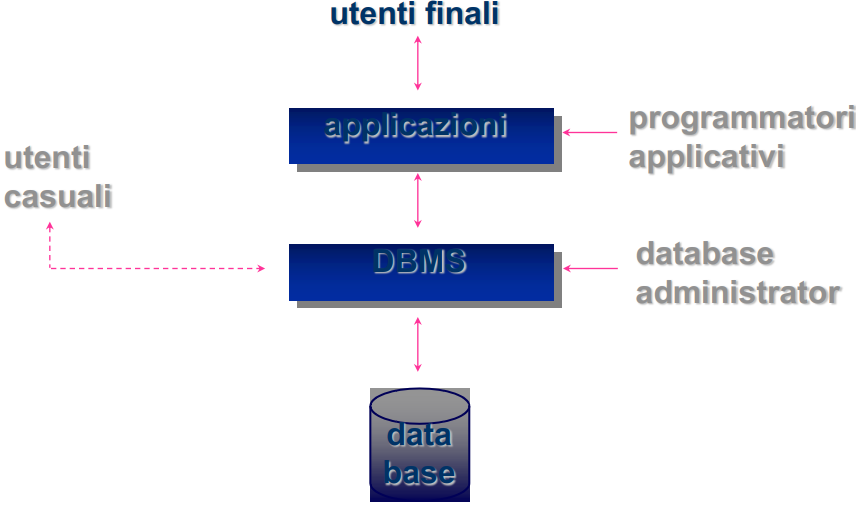
\includegraphics[width = 0.75\textwidth]{Images/10.PNG}
\end{center}
\subsection{Vantaggi e svantaggi dei DBMS}
Vediamo quali sono i \textbf{vantaggi} di avere un DBMS:
\begin{itemize}
    \item Permettono di considerare i dati come risorsa comune di un'organizzazione, a disposizione di molteplici applicazioni e utenti
    \item Offrono un modello della parte di mondo di interesse che è unificato e preciso, utilizzabile in applicazioni attuali e future
    \item Offrono un controllo centralizzato dei dati, riducendo ridondanze e inconsistenze
    \item Permettono l'indipendenza dei dati: favoriscono lo sviluppo di applicazioni flessibili e facilmente modificabili
\end{itemize}
Vediamo quali sono invece gli \textbf{svantaggi} di avere un DBMS:
\begin{itemize}
    \item Un DBMS è costoso, complesso e ha specifici requisiti in termini di software e hardware
    \item Diventa difficile separare, tra tutti i servizi offerti da un DBMS, quelli effettivamente usati da quelli inutili
    \item Sono inadatti alla gestione di applicazioni con pochi utenti (NB: Dipende dai costi operativi)
\end{itemize}
\subsection{Caratteristiche dell'approccio con basi di dati}
L'approccio alla \textbf{rappresentazione dei dati tramite basi di dati} ha le seguenti caratteristiche:
\begin{itemize}
    \item \textbf{Astrazione dei dati}: si usa un \textbf{modello dati} per nascondere dettagli e presentare all'utente una \textit{vista concettuale} del database
    \item \textbf{Supporto di viste multiple dei dati}: Ogni utente può usare una vista (view) differente del database, contente solo i dati di interesse per quell'utente
\end{itemize}
\section{Progettazione di unaa base di dati}
La \textbf{progettazione di basi di dati} è una delle attività del processo di sviluppo dei sistemi informativi e va quindi inquadrata in un contesto più generale: \textbf{il ciclo di vita dei sistemi informativi}.
\subsection{Ciclo di vita dei sistemi informativi}
Il ciclo di vita dei sistemi informativi è \textbf{l'insieme e sequenzializzazione delle attività svolte da analisti, progettisti, utenti nello sviluppo e nell'uso dei sistemi informativi}.
È un attività iterativa, quindi è un "ciclo".
\newpage
\noindent
Le fasi del ciclo di vita sono:
\begin{center}
    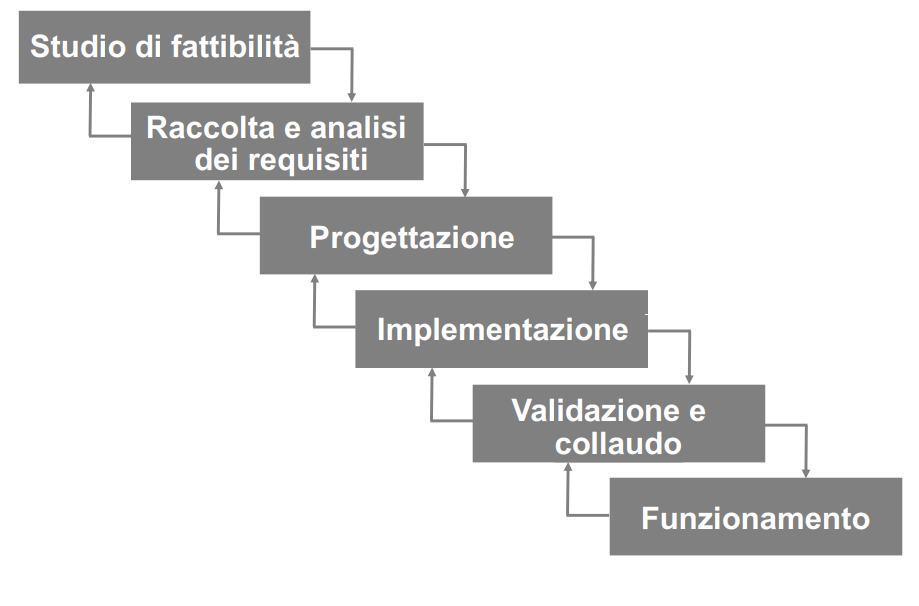
\includegraphics[width = 0.85\textwidth]{Images/11.PNG}
\end{center}
Diamone una definizione:
\begin{itemize}
    \item \textbf{Studio di fattibilità}: definizione dei costi e delle priorità
    \item \textbf{Raccolta e analisi dei requisiti}: studio delle proprietà del sistema
    \item \textbf{Progettazione}: di dati e funzioni
    \item \textbf{Validazione e collaudo}: sperimentazione
    \item \textbf{Funzionamento}: il sistema diventa operativo
\end{itemize}
Possiamo anche rappresentare questo ciclo di vita come una spirale:
\begin{center}
    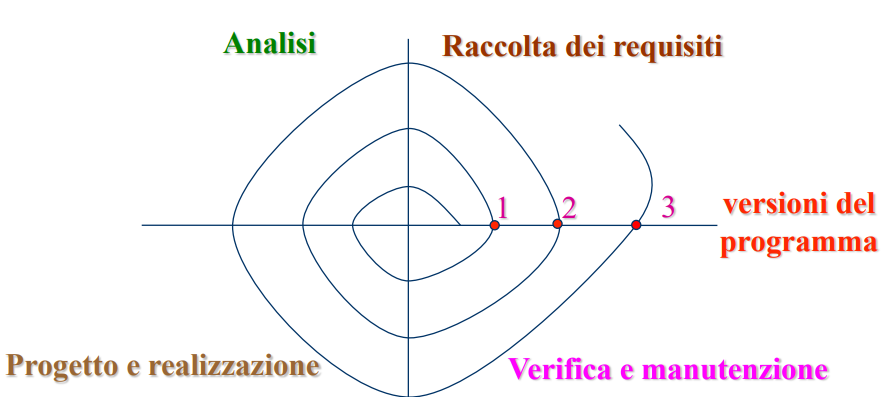
\includegraphics[width = 0.85\textwidth]{Images/12.PNG}
\end{center}
\subsubsection{Progettazione}
La progettazione dei dati individua l'organizzazione e la struttura della base di dati.
La progettazione delle applicazioni schematizza le operazioni sui dati e progetta il software applicativo.
I dati hanno \textbf{un ruolo centrale} e grazie alla progettazione:
\begin{itemize}
    \item i dati sono \textbf{più stabili}
    \item Si progetta prima la base di dati e poi le applicazioni
\end{itemize}
\subsubsection{Metodologia di progettazione}
Per garantire prodotti di buona qualità è opportuno seguire \textbf{una metodologia di progetto}; cioè un'articolazione in fasi/passi di guida ad una attività di progettazione.
Serve una metodologia di progettazione (insieme di strumenti) che:
\begin{itemize}
    \item permetta di \textbf{suddividere} la progettazione in fasi successive indipendenti
    \item fornisca \textbf{strategie} da seguire e criteri di scelta in caso di alternative
    \item fornisca \textbf{modelli di riferimento (linguaggi)} per descrivere la realtà che stiamo progettando
\end{itemize}
e che garantisca:
\begin{itemize}
    \item \textbf{Generalità} rispetto ai problemi da affrontare
    \item \textbf{Qualità} in termini di correttezza, completezza ed efficienza
    \item \textbf{Facilità d'uso}
\end{itemize}
Una metodologia di progettazione di basi di dati si basa su un principio semplice ma efficace:
\textbf{la separazione netta tra decisioni relative a}:
\begin{itemize}
    \item \textbf{Come rappresentare}
    \item \textbf{Come farlo}
\end{itemize}
\begin{center}
    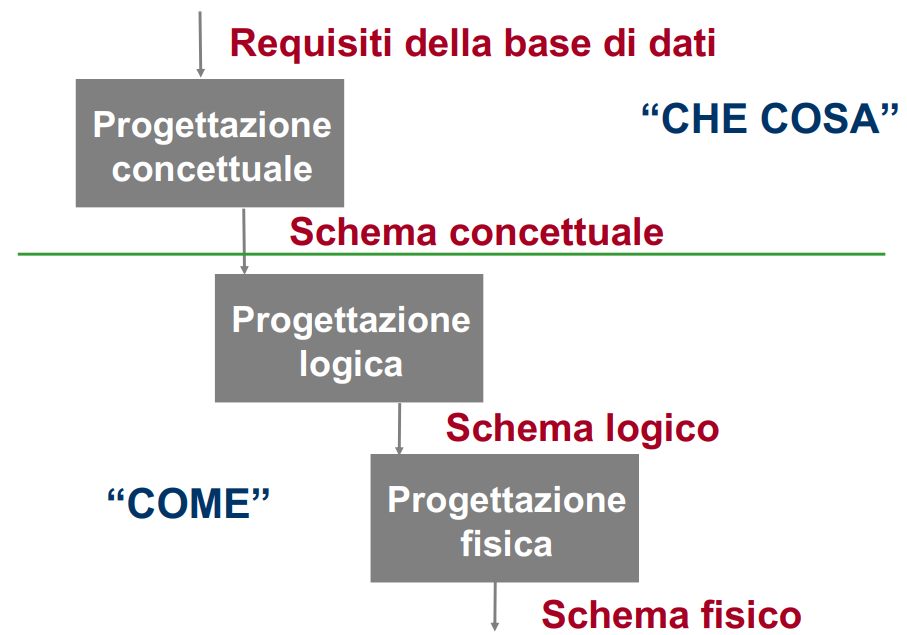
\includegraphics[width = 0.80\textwidth]{Images/13.PNG}
\end{center}
La metodologia introdotta prevede 3 fasi:
\begin{itemize}
    \item Progettazione \textbf{concettuale}
    \item Progettazione \textbf{logica}
    \item Progettazione \textbf{fisica}
\end{itemize}
Ognuna delle fasi si basa su un \textbf{modello}, che permette di generare una rappresentazione formale (schema) della base di dati ad un dato livello di astrazione (concettuale, logico e fisico):
\begin{itemize}
    \item Schema concettuale
    \item Schema logico
    \item Schema fisico
\end{itemize}
\subsubsection{Fase di progettazione concettuale}
La fase diu progettazione concettuale traduce i requisiti del sistema informatico in una descrizione \textbf{formalizzata e integrata} delle esigenze aziendali, espressa in modo \textbf{indipendente} dalle scelte implementative (DBMS, SW e HW).
Essa è:
\begin{itemize}
    \item \textbf{Formale}: la descrizione deve essere espressa con un linguaggio non ambiguo e capace di descrivere in modo soddisfacente il sistema analizzato
    \item \textbf{Integrata}: la descrizione deve essere in grado di descrivere nella globalità l'ambiente analizzato
    \item \textbf{Indipendente dall'ambiente tecnologico}: la descrizione deve concentrarsi sui dati e sulle loro relazioni e non sulle scelte implementative
\end{itemize}
\subsubsection{Fase di progettazione logica}
La progettazione logica consiste nella traduzione dello schema concettuale nel modello dei dati del DBMS.
Il risultato è uno schema logico, espresso nel DDL del DBMS.
In questa fase si considerano anche aspetti legati ai vincoli e all'efficienza.
La progettazione logica si articola in due sotto-fasi:
\begin{itemize}
    \item \textbf{Ristrutturazione dello schema concettuale}
    \item \textbf{Traduzione verso il modello logico}
\end{itemize}
\subsubsection{Progettazione fisica}
La progettazione fisica completa lo schema logico ottenuto con le specifiche proprie dell'hw/sw scelto.
Il risultato è lo \textbf{schema fisico} che descrive le strutture di memorizzazione ed accesso ai dati.
\subsubsection{Vantaggi della progettazione concettuale}
La progettazione concettuale permette una descrizione dei dati indipendete degli aspetti tecnologici con un livello di astrazione intermedio fra utente e sistema.
\textbf{Prevale l'aspetto intensionale}.
Inoltre, essa utilizza una rappresentazione prevalentemente \textbf{grafica}, che migliora la comunicazione tra i progettisti, gli utenti e tutte le persone coinvolte nella realizzazione dell'applicazione.
È inoltre utile per la \textbf{documentazione}.
\begin{center}
    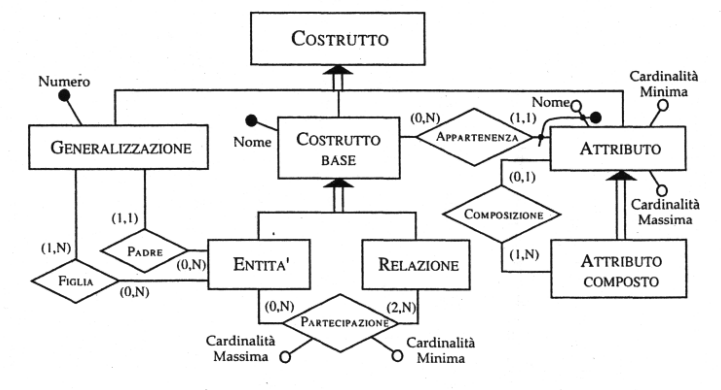
\includegraphics[width = 0.80\textwidth]{Images/14.PNG}
\end{center}
\section{Modello Entità-Relazione (E-R)}
Il modello entità-relazione (E-R) è un linguaggio grafico semi-formale per la rappresentazione di schemi concettuali.
Il modello E-R si è ormai affermato come uno standard nelle metodologie di progetto e nei sistemi SW di ausilio alla progettazione.
Ne esistono molte versione più o meno diverse l'una dall'altra.
\subsection{Introduzione ai costrutti}
\begin{center}
    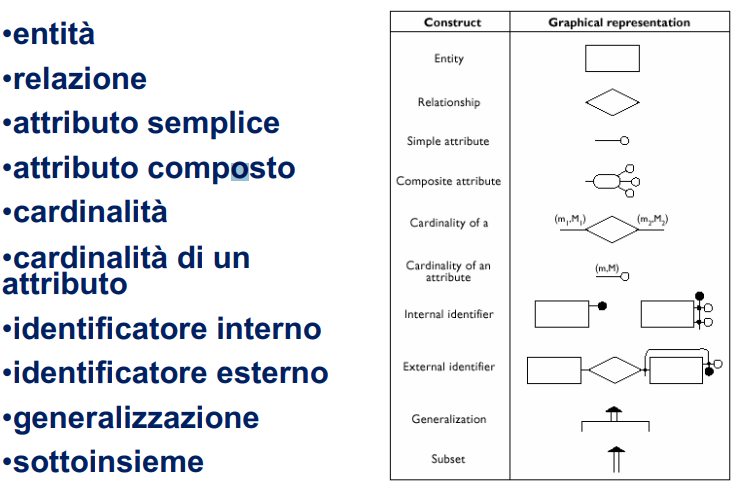
\includegraphics[width = 0.81\textwidth]{Images/15.PNG}
\end{center}
\subsection{Entità}
Un'entità è una classe di oggetti (fatti, persone, cose) della applicazione di interesse con proprietà comuni e con esistenza \textbf{autonoma} e della quale si vogliono registrare fatti specifici.
Per esempio, un'entità potrebbe essere un impiegato, un dipartimento, una città, un conto corrente, un'università, uno studente, ...
Graficamente le entità si rappresentano nel seguente modo:
\begin{center}
    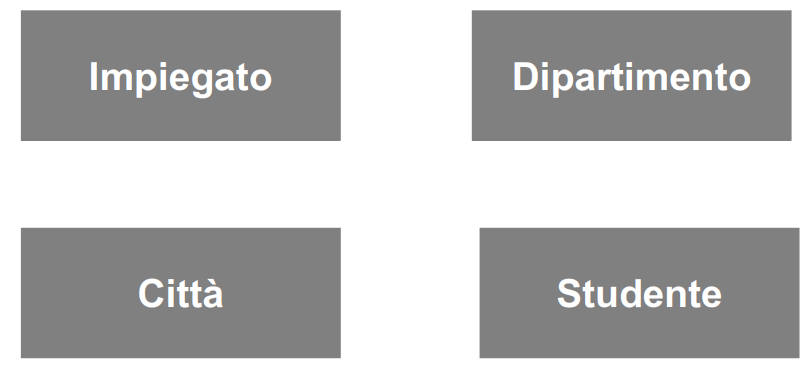
\includegraphics[width = 0.70\textwidth]{Images/16.PNG}
\end{center}
Ogni entità ha un nome che la identifica univocamente nello schema, il quale deve essere:
\begin{itemize}
    \item \textbf{Espressivo}
    \item \textbf{Al singolare}
\end{itemize}
A livello \textbf{estensionale} un'entità è costituita da un insieme di oggetti, che sono chiamati le sue \textbf{istanze}.
Ciò significa che, se in uno schema $S$ è definita una entità $E$, in ogni istanza $I$ dello schema $S$, alla entità $E$ è associato un insieme di oggetti
$$istanze(I,E) = \{e_1, e_2, e_3, \dots\}$$
che viene detto anche \textit{l'estensione} di $E$ nella istanza $I$ dello schema $S$.
Una istanza di entità non è un valore che identifica un oggetto, ma è \textbf{l'oggetto stesso}.
Quindi ogni istanza di entità è \textbf{oggetto della classe che l'entità rappresenta}.
Nello schema concettuale rappresentiamo le \textbf{entità}, non le singole istanze ("astrazione").
Quindi:
\begin{itemize}
    \item \textbf{Conoscenza astratta}: entità
    \item \textbf{Conoscenza concreta}: istanza di entità
\end{itemize}
\subsection{Attributi}
Un attributo di entità è una proprietà locale di un'entità, di interesse ai fini dell'applicazione.
Un attributo associa ad ogni istanza di entità un valore appartenente ad un insieme detto \textbf{dominio dell'attributo} (tipicamente interi, caratteri, stringhe, ecc\dots).
Si definisce quindi un attributo per l'entità $E$ quando si vuole rappresentare una proprietà \textbf{locale} delle istanze dell'entità $E$.
Una proprietà di un oggetto si dice locale quando in ogni istanza dello schema il valore di tale proprietà dipende \textbf{solamente} dall'oggetto stesso e \textbf{non ha alcun rapporto} con altri elementi dell'istanza dello schema.
Nel modello E-R, gli attributi si rappresentano nella seguente maniera:
\begin{center}
    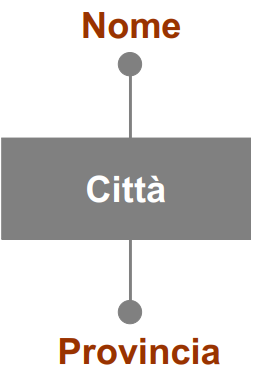
\includegraphics[width = 0.25\textwidth]{Images/17.PNG}
\end{center}
Ogni attributo di entità ha un nome che lo identifica in modo univoco nell'ambito dell'entità, ed è rappresentato da un cerchio collegato alla entità a cui appartiene.
Ogni attributo è definito su un dominio di valori. Un attributo associa ad ogni istanza di entità o associazione un valore nel corrispondente dominio.
I domini solitamente non vengono specificati nell'E-R ma nella documentazione associata. Se li si vuole indicare, la notazione è la seguente:
\begin{center}
    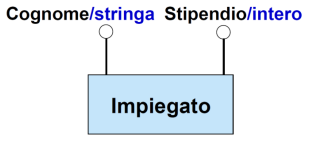
\includegraphics[width = 0.50\textwidth]{Images/18.PNG}
\end{center}
Quindi, ogni attributo può essere pensato come una vera e propria \textbf{funzione} che associa una determinata istanza di un'entità ad un particolare valore per quell'attributo;
di conseguenza \textbf{valgono tutte le definizioni e tutte le proprietà delle funzioni}
\begin{center}
    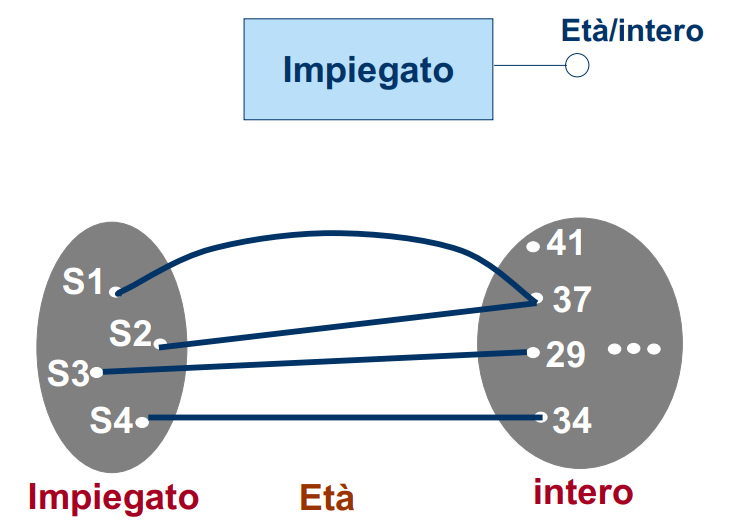
\includegraphics[width = 0.65\textwidth]{Images/19.PNG}
\end{center}
Inoltre, un'attributo è una \textbf{funzione totale}, quindi ogni istanza di un'entità deve avere un valore associato per ogni suo attributo.
\subsection{Attributi composti}
Gli attributi composti si ottengono raggruppando attributi di una medesima entità o relazione che presentano affinità nel loro significato o uso:
\begin{center}
    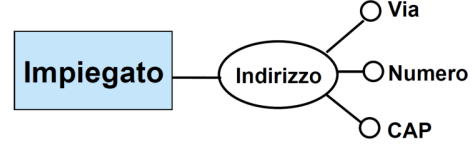
\includegraphics[width = 0.40\textwidth]{Images/20.PNG}
\end{center}
\subsection{Relazioni}
Una relazione è un fatto che descrive un'azione o una situazione che \textbf{stabilisce legami logici} tra istanze di entità (associa, mette in relazione) nella
\textbf{realtà che stiamo considerando}.
\textbf{I legami possono essere fra più di due entità}. Il numero di entità coinvolte in una relazione determina il suo \textbf{grado}.
Nel modello E-R una relazione si indica nel seguente modo:
\begin{center}
    
\includegraphics[width = 0.65\textwidth]{Images/21.PNG}
\end{center}
Ogni relazione ha un nome che la identifica univocamente nello schema ed esso deve essere:
\begin{itemize}
    \item \textbf{Espressivo}
    \item \textbf{Singolare} e usare \textbf{sostantivi invece che verbi}
\end{itemize}
A livello \textbf{estensionale} una relazione $R$ tra le entità $E$ ed $F$ è costituita da un insieme di coppie $(x,y)$, tali che $x$ è una istanza di $E$ ed $y$ è un istanza di $F$.
Ogni coppia è detta \textbf{istanza} della relazione $R$.
cIò significa che, se in uno schema $S$ è definita una relazione $R$ sulle entità $E$ ed $F$, in ogni istanza $I$ dello schema $S$, alla relazione $R$ è associato un insieme di coppie
(denotato da istanze $(I, R)$)
$$\{(x_1, y_1) (x_2, y_2), (x_3, y_3), \dots\}$$
che viene detto anche \textit{l'estensione} di $R$ nella istanza $I$ dello schema $S$.
In altre parole, una relazione nel modello E-R è, dal punto di vista della semantica, una relazione matematica.
In ogni istanza $I$ dello schema $S$ si ha:
$$istanze(I, R) \subseteq istanze(I,E) \times istanze(I,F)$$
In particolare si dice \textbf{istanza di un'associazione} la combinazione (aggregazione) di istanze di entità che prendono parte alla associazione.
Dalla semantica delle relazioni segue immediatamente che \textbf{non} possono esistere due istanze della stessa relazione che coinvolgono le stesse istanze di entità.
\newpage
\noindent
Tuttavia \textbf{due entità possono essere coinvolte in più associazioni}:
\begin{center}
    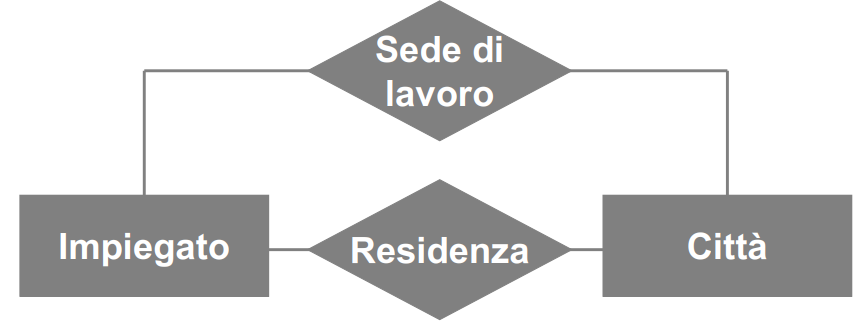
\includegraphics[width = 0.65\textwidth]{Images/22.PNG}
\end{center}
Inoltre le relazioni possono coinvolgere più di due entità:
\begin{center}
    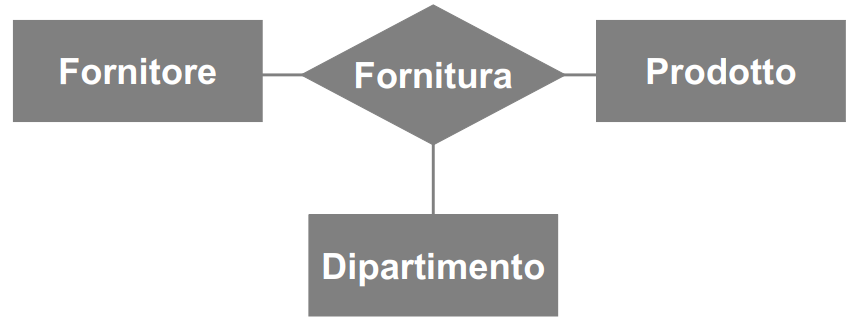
\includegraphics[width = 0.65\textwidth]{Images/23.PNG}
\end{center}
\begin{center}
    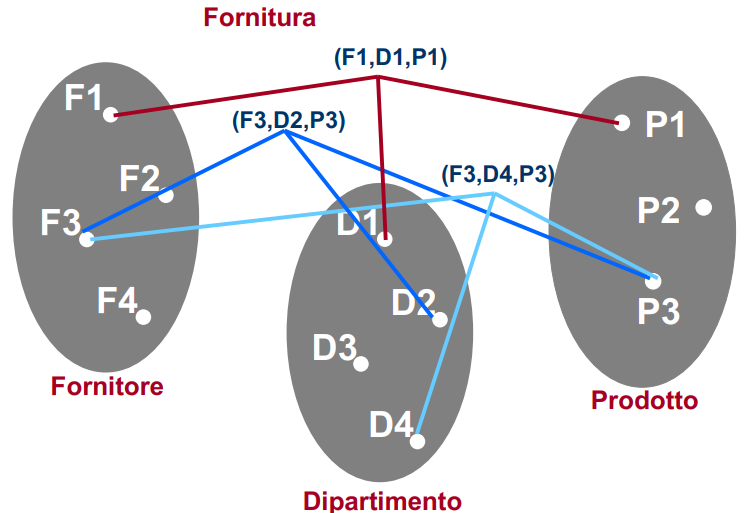
\includegraphics[width = 0.65\textwidth]{Images/24.PNG}
\end{center}
Se si parla quindi di una relazione \textbf{n-aria}, a livello \textbf{estensionale} (ovvero in ogni istanza $I$ dello schema $S$) una relazione $R$ tra le entità
$E_1, E_2, \dots, E_n$ è costituita dun insieme di n-uple (o tuple) $(x_1, x_2, \dots, x_n)$, tali che $x_1$ è un istanza di $E_1$ in $I$, $x_2$ è un istanza di $E_2$ in $I$, \dots
$x_N$ è un istanza di $E_n$ in $I$.
Ogni n-upla è detta \textbf{istanza} della relazione $R$ nella istanza $I$ dello schema $S$.
Quindi, in ogni istanza $I$ dello schema si ha:
$$istanze(I,R) \subseteq istanze(I, E_1) \times \dots \times istanze(I, E_n)$$
\subsection{Attributi di relazione}
Un attributo di relazione è una proprietà locale di una relazione, di interesse ai fini dell'applicazione.
Un attributo della relazione $R$ tra le entità $E_1, E_2, \dots, E_n$ modella una proprietà \textbf{non} propria delle entità
ma del \textbf{legame} tra le varie entità rappresentato da $R$.
Un attributo associa ad ogni istanza di relazione un valore appartenente ad un insieme detto \textbf{dominio} dell'attributo.
Ogni attributo di relazione ha un nome che lo identifica in modo univoco nell'ambito della relazione, ed è rappresentato da un cerchio collegato alla relazione a cui appartiene.
\begin{center}
    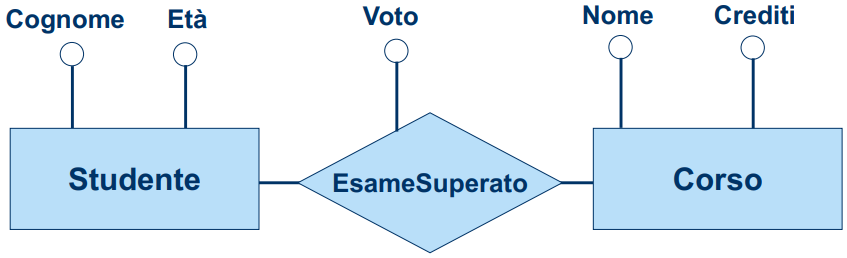
\includegraphics[width = 0.70\textwidth]{Images/25.PNG}
\end{center}
\begin{center}
    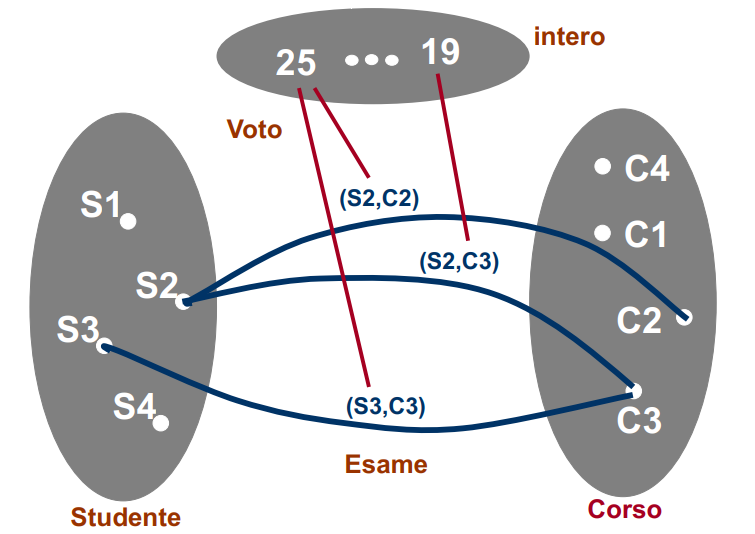
\includegraphics[width = 0.70\textwidth]{Images/26.PNG}
\end{center}
Ovviamente gli attributi possono essere presenti su associazioni n-arie:
\begin{center}
    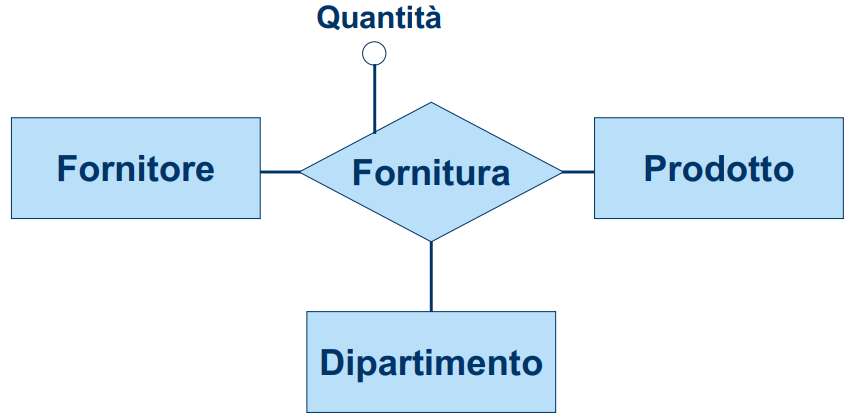
\includegraphics[width = 0.75\textwidth]{Images/27.PNG}
\end{center}
\begin{center}
    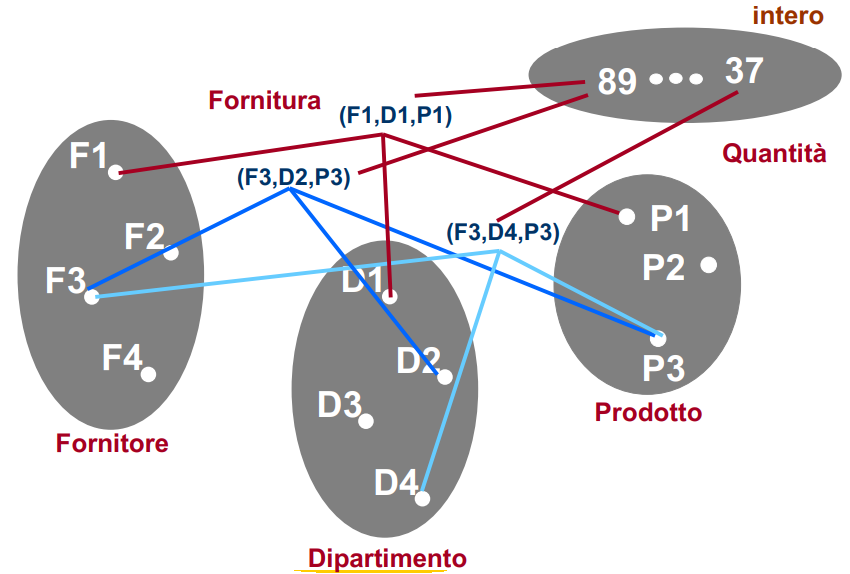
\includegraphics[width = 0.75\textwidth]{Images/28.PNG}
\end{center}
\subsection{Analisi dei casi dubbi}
I nomi di entità e associazioni alle volte traggono in inganno: è bene quindi, nel caso si presentino situazioni poco chiare, bisogna provare a ragionare anche in termini di istanze:
cosa "contiene" effettivamente questa entità/associazione?
\subsection{Relazioni ricorsive}
Una associazione può coinvolgere "due o più volte" la stessa entità:
\begin{center}
    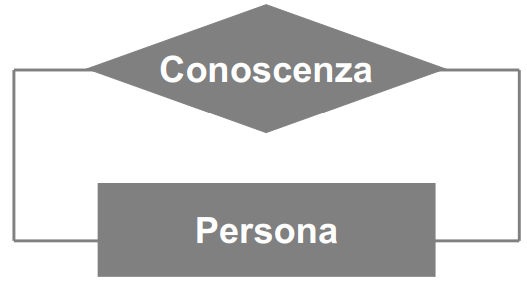
\includegraphics[width = 0.40\textwidth]{Images/29.PNG}
\end{center}
Vi è però il problema di \textbf{identificare i ruoli in questa associazione}.
Per farlo, essi si scrivono di fianco ai "collegamenti" che collegano la relazione con l'entità:
\begin{center}
    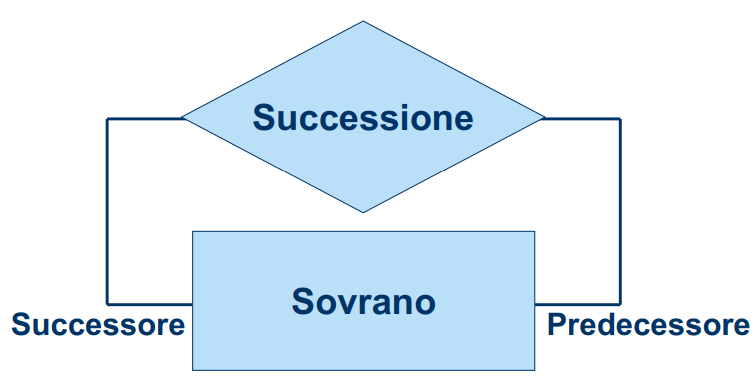
\includegraphics[width = 0.60\textwidth]{Images/30.PNG}
\end{center}
\newpage
\noindent
Un'associazione ricorsiva può essere o meno:
\begin{itemize}
    \item \textbf{Simmetrica}: $(a,b) \in A \Rightarrow (b,a) \in A$
    \item \textbf{Riflessiva}: $(a,a) \in A$
    \item \textbf{Transitiva}: $(a,b) \in A, (b,c) \in A \Rightarrow (a,c) \in A$
\end{itemize}
Una associazione ricorsiva può essere anche n-aria:
\begin{center}
    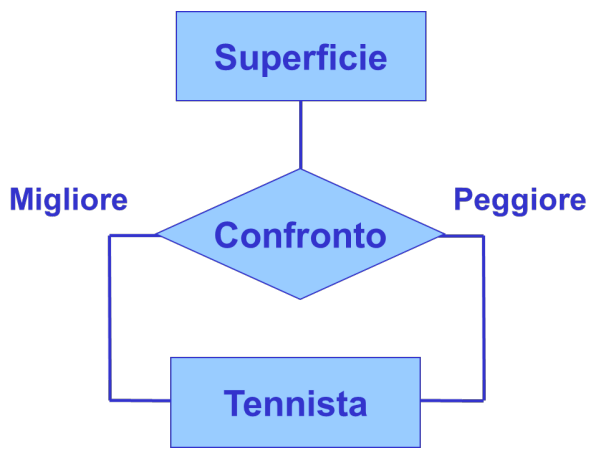
\includegraphics[width = 0.30\textwidth]{Images/31.PNG}
\end{center}
\subsection{Scelta tra entità, relazione e attributo}
Un concetto verrà modellato come:
\begin{itemize}
    \item \textbf{Entità}:
    \begin{itemize}
        \item Se le sue istanze sono concettualmente significative indipendentemente da altre istanze
        \item Se ha o potrà avere delle proprietà indipendenti dagli altri concetti
        \item Se il concetto è importante nell'applicazione
    \end{itemize}
    \item \textbf{Attributo} di un'entità o di una relazione:
    \begin{itemize}
        \item Se le sue istanze non sono concettualmente significative
        \item Se non ha senso considerare una sua istanza indipendentemente da altre istanze
        \item Se serve solo a rappresentare una proprietà locale di un altro concetto
    \end{itemize}
    \item \textbf{Relazione}:
    \begin{itemize}
        \item Se le sue istanze non sono concettualmente significative indipendentemente da altre istanze, cioè le sue istanze rappresentano n-uple di altre istanze
        \item Se non ha senso pensare alla partecipazione delle sue istanze ad altre relazioni
    \end{itemize}
\end{itemize}
Le scelte che si prendono possono cambiare durante l'analisi.
\subsection{Cardinalità}
La cardinalità è una coppia di valori che si associa a ogni entità che partecipa a una relazione.
Specificano il numero minimo e massimo di occorrenze della relazione cui ciascuna occorrenza di una entità può partecipare.
Per semplicità usiamo solo tre simboli:
\begin{itemize}
    \item 0 e 1 per la cardinalità \textbf{minima}
    \begin{itemize}
        \item 0 = "partecipazione \textbf{opzionale}"
        \item 1 = "partecipazione \textbf{obbligatoria}"
    \end{itemize}
    \item 1 e "N" per la \textbf{massima}; con N che non pone alcun limite
\end{itemize}
Nel modello E-R le cardinalità si rappresentano nel seguente modo:
\begin{center}
    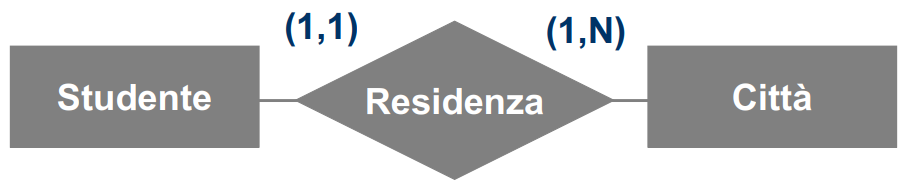
\includegraphics[width = 0.65\textwidth]{Images/32.PNG}
\end{center}
Con riferimento alle cardinalità \textbf{massime}, abbiamo relazioni:
\begin{itemize}
    \item \textbf{Uno a uno}: se le cardinalità massime di entrambe le entità sono uno
    \item \textbf{Uno a molti}: se la cardinalità massima associata ad un'entità è 1 e la cardinalità massima associata all'altra entità è N 
    \item \textbf{Molti a molti}: se le cardinalità massime per entrambe le entità è N
\end{itemize}
\subsubsection{Vincoli di cardinalità}
Un \textbf{vincolo di cardinalità} tra un'entità $E$ e una relazione $R$ esprime un limite minimo (\textbf{cardinalità minima})
ed un limite massimo (\textbf{cardinalità massima}) di istanze della relazione $R$ a cui può partecipare ogni istanza dell'entità $E$.
Serve a caratterizzare meglio il significato di una relazione.
\subsubsection{Cardinalità di attributi}
È possibile associare delle cardinalità anche agli attributi, con due scopi:
\begin{itemize}
    \item Indicare \textbf{opzionalità}
    \item Indicare \textbf{attributi multivalore}
\end{itemize}
\begin{center}
    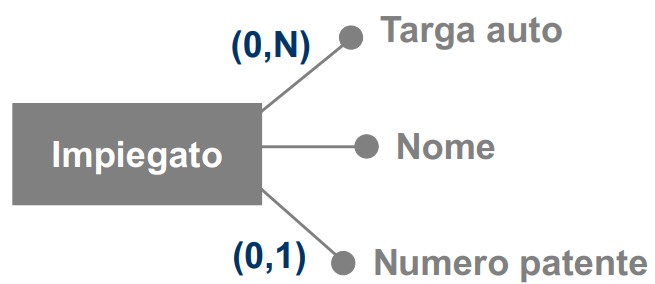
\includegraphics[width = 0.65\textwidth]{Images/33.PNG}
\end{center}
\subsection{Identificatori di un'entità}
L'identificatore è uno "strumento" per l'identificazione univoca delle occorrenze di un'entità.
Esso è costituito da
\begin{itemize}
    \item \textbf{Attributi dell'entità}; in questo caso è detto \textbf{identificatore interno}
    \item \textbf{Attributi dell'entità più entità esterne attraverso relazioni}; in questo caso è detto \textbf{identificatore esterno}
\end{itemize}
Per gli \textbf{identificatori interni} si segue la seguente notazione:
\begin{itemize}
    \item Se l'identificatore è formato da un solo attributo, si annerisce il corrispondente pallino
    \item Se l'identificatore è formato da più attributi, si uniscono gli attributi con una linea che termina con pallino annerito
\end{itemize}
\begin{center}
    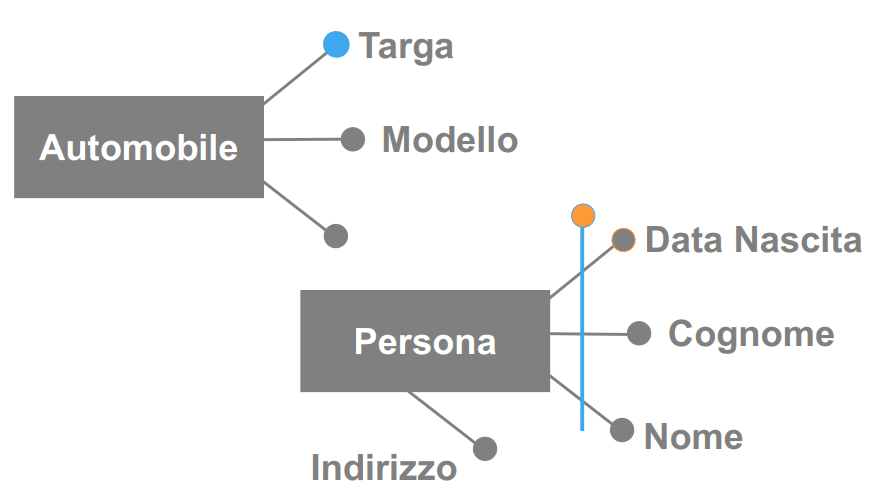
\includegraphics[width = 0.65\textwidth]{Images/34.PNG}
\end{center}
Per gli \textbf{identificatori esterni} si segue la seguente notazione:
\begin{itemize}
    \item Se l'identificatore è formato da attributi e relazioni (o meglio, ruoli), si indica unendo gli attributi ed i ruoli con una linea che termina con pallino annerito.
    \item Una identificazione esterna è possibile solo \textbf{attraverso una relazione a cui l'entità da identificare partecipa con cardinalità (1,1)}
\end{itemize}
\begin{center}
    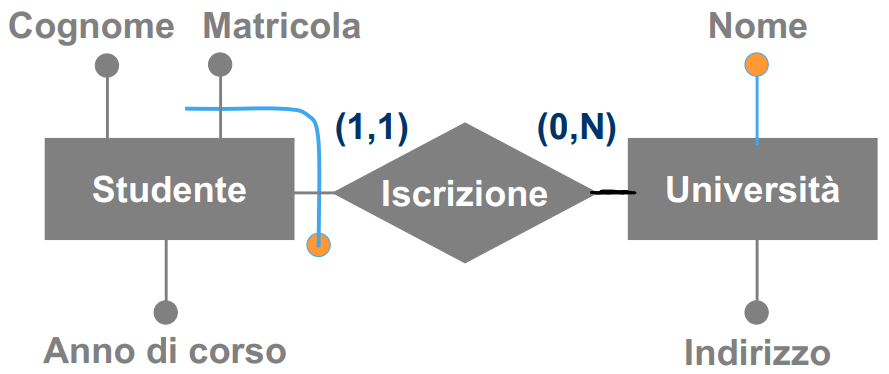
\includegraphics[width = 0.65\textwidth]{Images/35.PNG}
\end{center}
Ogni entità deve possedere almeno un identificatore, ma può averne in generale più di uno.
\subsection{Relazione IS-A tra entità}
Fino ad ora non abbiamo detto nulla sul fatto se due entità possano o no avere istanze in comune.
È facile verificare che, in molti contesti, può accadere che tra due classi rappresentate da due entità nello schema concettuale sussista la \textbf{relazione IS-A} (o relazione di sottoinsieme), e cioè che \textbf{ogni istanza di una sia anche istanza dell'altra}.
(Es. Studente, Studente della laurea breve).
La relazione IS-A nel modello E-R si può definire tra due entità, che si dicono rispettivamente "entità padre" ed "entità figlia" (o sottoentità, cioè quella che rappresenta un sottoinsieme dell'entità padre).
La relazione IS-A si rappresenta nel diagramma dello schema concettuale nel seguente modo:
\begin{center}
    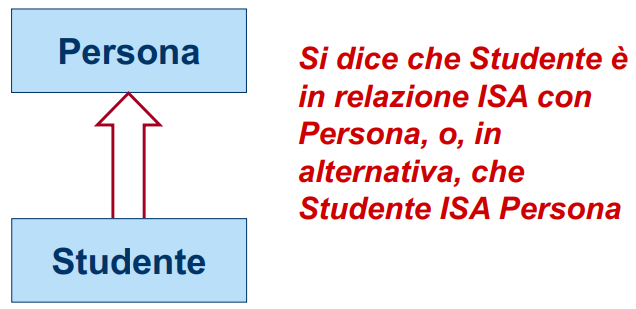
\includegraphics[width = 0.50\textwidth]{Images/36.PNG}
\end{center}
\subsubsection{Ereditarietà su entità}
La relazione IS-A implica il \textbf{principio di ereditarietà}: ongi proprietà dell'entità padre è anche una proprietà della sottoentità, e non si riporta esplicitamente nel diagramma.
L'entità figlia può avere ovviamente ulteriori proprietà.
\subsection{Generalizzazione tra entità}
Finora, abbiamo considerato la relazione IS-A che stabilisce che l'entità padre è più generale della sottoentità.
Talvolta, però, l'entità padre può generalizzare diverse sottoentità rispetto ad un unico criterio. In questo caso si parla di \textbf{generalizzazione}.
Nella generalizzazione, le sottoentità hanno insiemi di istanze disgiunti a coppie (anche se in alcune varianti del modello E-R, si può specificare se due sottoentità della stessa entità padre sono disgiunte o no).
Una generalizzazione può essere di due tipi:
\begin{itemize}
    \item \textbf{Completa}: l'unione delle istanze delle sottoentità è uguale all'insieme delle istanze dell'entità padre; si indica con una freccia annerita
    \item \textbf{Non completa}: si indica con una freccia non riempita
\end{itemize}
Alla generalizzazione si associa una coppia di lettere che indica come interpretare la generalizzazione.
La prima lettera indica il tipo di generalizzazione e può assumere i valori:
\begin{itemize}
    \item \textbf{t} per le generalizzazione complete (totali)
    \item \textbf{p} per le generalizzazioni non complete (parziali)
\end{itemize}
\newpage
\noindent
La seconda lettera invece indica se le sottoentità si sovrappongono o meno; essa può assumere i valori:
\begin{itemize}
    \item \textbf{e} se le sottoentità non si sovrappongono (esclusiva)
    \item \textbf{s} se le sottoentità si sovrappongono (sovrapposte)
\end{itemize}
\begin{center}
    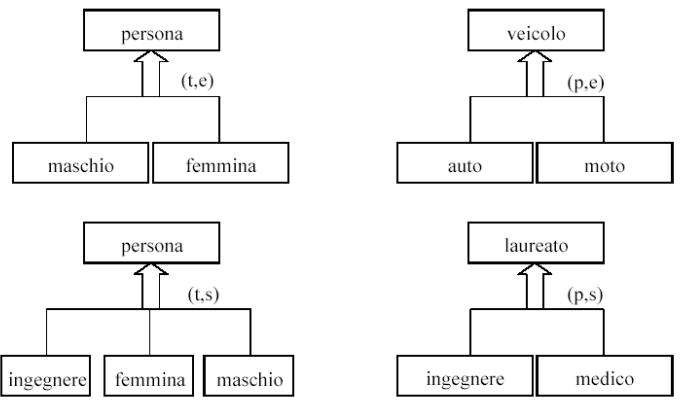
\includegraphics[width = 0.77\textwidth]{Images/37.PNG}
\end{center}
Nel modello E-R vige la regola che una entità può avere \textbf{al massimo una} entità padre. In altre parole, il modello E-R \textbf{non ammette ereditarietà multipla}.
Ovviamente, quando si contano i padri di una sottoentità si tiene conto anche di eventuali relazioni \textbf{IS-A} che essa ha con altre entità.
\begin{center}
    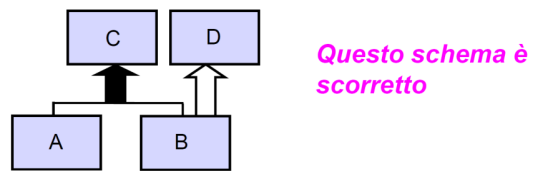
\includegraphics[width = 0.60\textwidth]{Images/38.PNG}
\end{center}
\subsubsection{Generalizzazioni ed ereditarietà}
Il \textbf{principio di ereditarietà} vale anche per le generalizzazioni: ogni proprietà dell'entità padre è anche una proprietà della sottoentità, e non si riporta esplicitamente nel diagramma.
L'entita figlia può avere ovviamente ulteriori proprietà.
\subsubsection{Diverse generalizzazioni della stessa classe}
La stessa entità può essere padre in diverse generalizzazioni.
Concettualmente, non c'è alcuna correlazione tra due generalizzazioni diverse, perché rispondono a due criteri diversi di classificare le istanze delle entità padre.
\subsubsection{Differenza tra due IS-A e una generalizazione}
Ci si potrebbe chiedere se non si possa utilizzare due IS-A per rappresentare una generalizzazione.
In realtà, le due (o più) sottoclassi che derivano da una generalizzazione derivano da uno stesso criterio di classificazione delle istanze della superclasse.
Le due sottoentità di due IS-A differenti invece sono indipendenti, nel senso che il loro significato non deriva dallo stesso criterio di classificazione delle istanze della entità padre.
\subsubsection{Altre proprietà}
Vi sono altre proprietà della generalizzazione:
\begin{itemize}
    \item Possono esistere gerarchie a più livelli e multiple generalizzazioni allo stesso livello
    \item Un'entità può essere inclusa in più gerarchie, come genitore e/o come figlia
    \item Se una generalizzazione ha solo un'entità figlia, si parla di \textbf{sottoinsieme}
\end{itemize}
\subsection{Relazione IS-A fra relazioni}
Nel caso di una relazione IS-A fra relazioni la semantica non cambia rispetto al caso della relazione IS-A tra entità:
se in uno schema $S$ è definita la relazione IS-A tra $R$ e $Q$ ($R$ IS-A $Q$, dove $R$ e $Q$ sono due relazioni con lo stesso grado e gli stessi ruoli), allora
in ogni istanza $I$ dello schema $S$, si ha che
$$istanze(I, R) \subseteq istanze(I, Q)$$
\begin{center}
    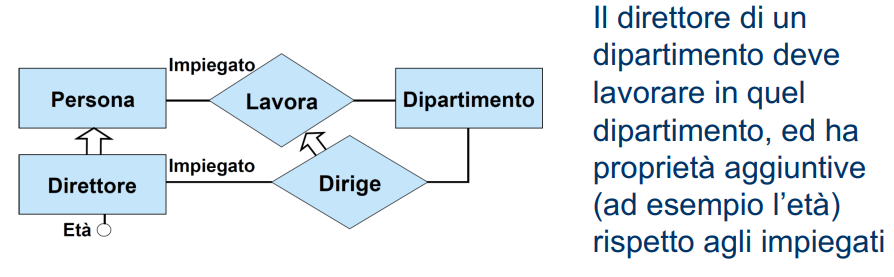
\includegraphics[width = 0.90\textwidth]{Images/39.PNG}
\end{center}
\subsection{Vincoli non esprimibili nel diagramma E-R}
Gli schemi E-R permettono di cogliere la maggior parte delle interrelazioni tra i dati del dominio d'interesse.
Tuttavia alcune interrelazioni non possono essere colte direttamente da uno schema E-R.
Talli interrelazioni vanno in ogni caso tenute presenti attraverso delle asserzioni aggiuntive dette \textbf{vincoli esterni al diagramma}, o semplicemente, \textbf{vincoli esterni}.
Come rappresentiamo tali vincoli?
\begin{itemize}
    \item Attraverso formalismi opportuni (es. \textbf{logica matematica})
    \item Attraverso asserzioni in linguaggio naturale (che devono essere il più possibile \textbf{precise e non ambigue})
\end{itemize}
\subsection{Documentazione associata agli schemi E-R}
Oltre al diagramma E-R, lo schema concettuale è descritto dal cosiddetto \textbf{dizionario dei dati}: esso è costituito dalle tabelle di
\begin{itemize}
    \item Entità
    \item Relazioni 
    \item Attributi 
    \item Vincoli esterni
\end{itemize}
\begin{center}
    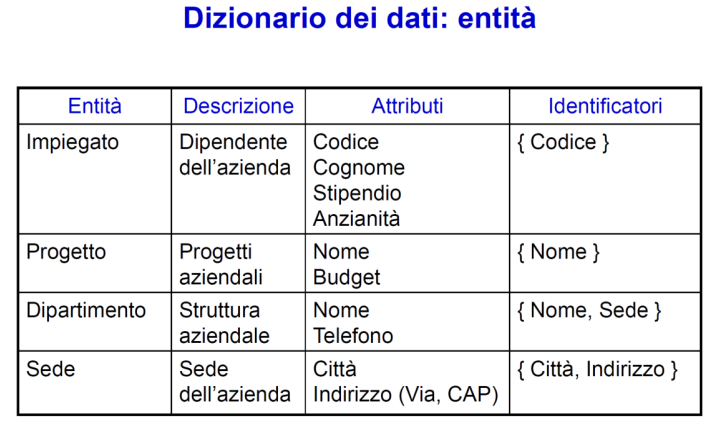
\includegraphics[width = 0.75\textwidth]{Images/40.PNG}
\end{center}
\begin{center}
    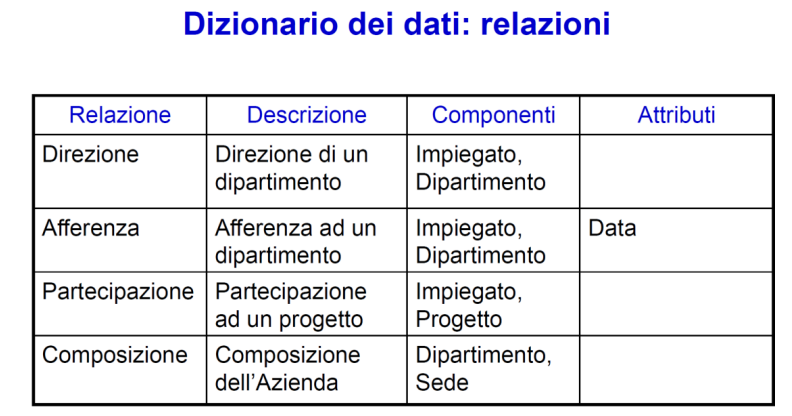
\includegraphics[width = 0.80\textwidth]{Images/41.PNG}
\end{center}
\begin{center}
    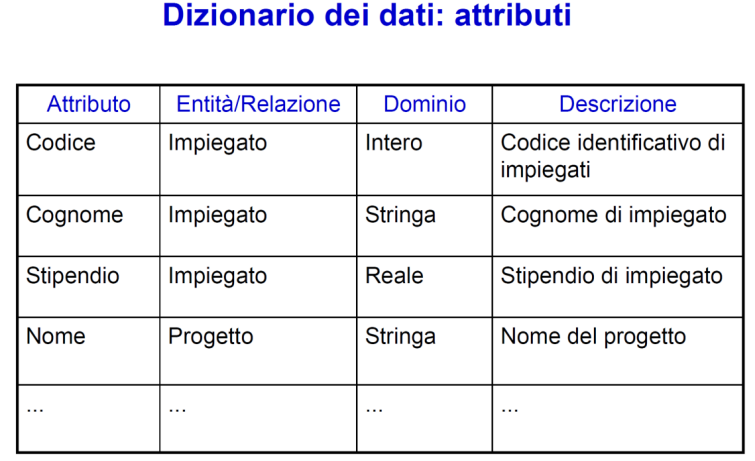
\includegraphics[width = 0.75\textwidth]{Images/42.PNG}
\end{center}
\begin{center}
    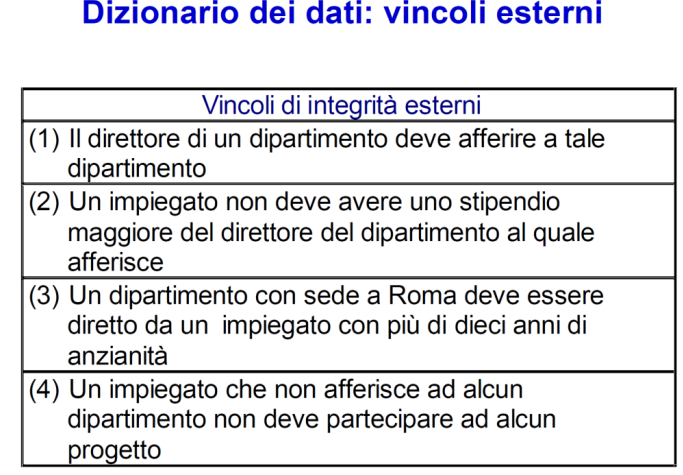
\includegraphics[width = 0.75\textwidth]{Images/43.PNG}
\end{center}
In particolare, il dizionario dei vincoli esterni può avere, a sua volta, altri vincoli esterni espressi in un altro dizionario.
\section{Progettazione concettuale}
L'analisi dei requisiti e la progettazione concettuale ("analisi dei dati") comprende attività interconnesse di:
\begin{itemize}
    \item Acquisizione dei requisiti
    \item Analisi dei requisiti
    \item Costruzione dello schema concettuale
    \item Costruzione del glossario
\end{itemize}
Per i requisti, possibili fonti sono:
\begin{itemize}
    \item \textbf{Utenti}, attraverso:
    \begin{itemize}
        \item Interviste
        \item Documentazione apposita
    \end{itemize}
    \item \textbf{Documentazione esistente}
    \begin{itemize}
        \item Normative (leggi, regolamenti di settore)
        \item Regolamenti interni, procedure aziendali
        \item Realizzazioni preesistenti
    \end{itemize}
    \item \textbf{Modulistica}
\end{itemize}
Il reperimento dei requisiti è un 'attività difficile e non standardizzabile. L'attività di anlisi iniza con i primi requisiti raccolti e spesso indirizza verso altre acquisizioni.
\begin{center}
    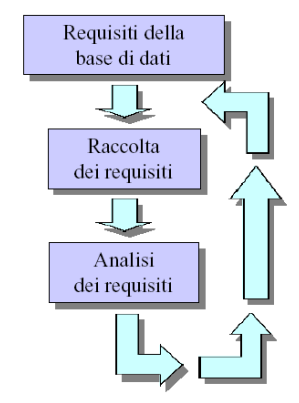
\includegraphics[width = 0.35\textwidth]{Images/44.PNG}
\end{center}
\subsection{Requisiti}
\subsubsection{Acquisizione per interviste}
Utenti diversi possono fornire informazioni diverse.
Utenti a livello più alto hanno spesso una visione più ampia ma meno dettagliata.
Le interviste portano spesso ad una acquisizione dei requisiti "per raffinamenti successivi".
\subsubsection{Interazione con gli utenti}
Spunti per ottenere requisiti tramite l'interazione con gli utenti possono essere:
\begin{itemize}
    \item Effettuare spesso verifiche di comprensione e coerenza
    \item Verificare anche per mezzo di esempi (generali e relativi ai casi limite)
    \item Richiedere definizioni e classificazioni
    \item Far evidenziare gli aspetti essenziali rispetto a quelli marginali
\end{itemize}
\subsubsection{Documentazione descrittiva}
Le regole generali sono:
\begin{itemize}
    \item Scegliere il corretto livello di astrazione
    \item Standardizzare la struttura delle frasi
    \item Suddividere le frasi articolate
    \item Separare le frasi sui dati da quelle sulle funzioni
\end{itemize}
\subsubsection{Organizzazione di termini e concetti}
Le regole generali sono:
\begin{itemize}
    \item Costruire un glossario dei termini
    \item Individuare omonimi e sinonimi e unificare i termini
    \item Rendere esplicito il riferimento fra termini
    \item Riorganizzare le frasi per concetti
\end{itemize}
L'analisi dei requisiti procede per \textbf{raffinamenti successivi}.
\subsubsection{Scrittura dei requisiti}
Per scrivere correttamente i requisiti serve:
\begin{itemize}
    \item \textbf{Scegliere il livello di astrazione}: Si devono evitare termini troppo generici o troppo specifici
    \item \textbf{Standardizzare la struttura delle frasi}: È preferibile usare sempre lo stesso stile sintattico
    \item \textbf{Evitare frasi contorte}
    \item \textbf{Individuare sinonimi/omonimi e unificare i termini}: Usare un solo termine al posto dei sinonimi; usare termini distinti in caso di omonimi
    \item \textbf{Rendere esplicito il riferimento fra termini}: In assenza di un contesto di riferimento alcuni termini possono risultare ambigui. Occorre rappresentare il riferimento fra i termini
    \item \textbf{Costruire un glossario dei termini (facoltativo)}: per ogni termine si indica una breve descrizione, i sinonimi e gli altri termini con cui esiste un legame logico. Facilita la comprensione e la precisazione dei termini
\end{itemize}
\subsection{Specifiche sulle operazione}
Per scrivere le specifiche sulle operazioni occorre utilizzare la stessa terminologia utilizzata per le specifiche dei dati (glossario).
Serve anche conoscere la frequenza con la quale le operazioni sono eseguite.
\subsection{Dalle specifiche al modello E-R}
Per passare dalle specifiche al modello E-R si utilizzano le definizioni dei costrutti del modello E-R.
Se un concetto proprietà significative e descrive classi di oggetti con esistenza autonoma conviene rappresentarlo con una \textbf{entità}.
Se un concetto ha una struttura semplice e non possiede proprietà rilevanti associate conviene rappresentarlo come un \textbf{attributo} di un altro concetto a cui si riferisce.
Se sono state individuate due o più entità e nei requisiti compare un concetto che le associa, questo concetto può essere rappresentato con una \textbf{relazione}.
Se uno pià concetti risultano essere il caso particolare di un altro è opportuno rappresentarli facendo uso della \textbf{generalizzazione}.
\subsection{Design patterns}
I \textbf{design patterns} sono soluzioni progettuali a problemi comuni.
Sono largamente usati nell'ingegneria del software.
I design pattern per le basi di dati utilizzano il concetto di \textbf{reificazione}, cioè il procedimento di creazione di un modello dati su un concetto astratto predefinito.
\subsubsection{Reificazione di attributo di entità}
Questo design pattern estrae un attributo e lo rende entità poiché, nel contesto applicativo, esso ha dignità di entità
\begin{center}
    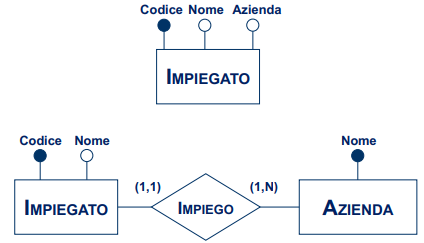
\includegraphics[width = 0.60\textwidth]{Images/45.PNG}
\end{center}
\subsubsection{Part-of}
A volte un'entità può essere legata a un'altra entità creando una relazione di tipo (1, N). Gli esempi
mostrano come il concetto di part-of possa essere di \textbf{dipendenza}.
\begin{center}
    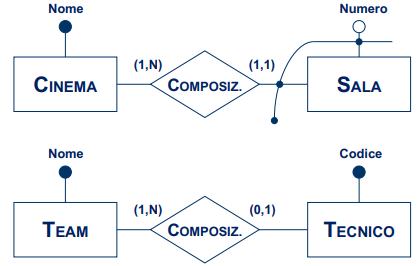
\includegraphics[width = 0.50\textwidth]{Images/46.PNG}
\end{center}
\subsubsection{Instance-of}
A volte si viene a creare la necessità di creare un'entità astratta che prenda concretezza in un'entità istanza.
\begin{center}
    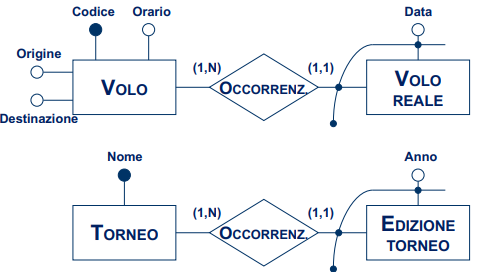
\includegraphics[width = 0.70\textwidth]{Images/47.PNG}
\end{center}
\subsubsection{Reificazione di relazione binaria}
\begin{center}
    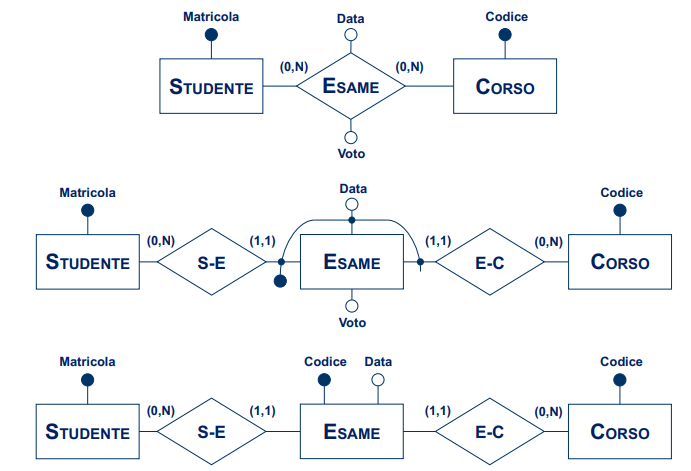
\includegraphics[width = 0.80\textwidth]{Images/48.PNG}
\end{center}
\subsubsection{Reificazione di relazione ricorsiva}
Nell'esempio, partita potrebbe essere vista come una relazione binaria tra squadra e se stessa.
\begin{center}
    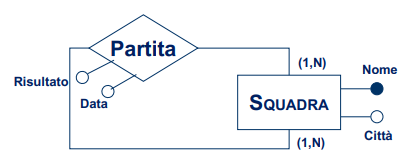
\includegraphics[width = 0.50\textwidth]{Images/49.PNG}
\end{center}
Come sappiamo una squadra può giocare più volte, reificare partita come nello schema seguente è più utile per esprimere questo concetto:
\begin{center}
    \includegraphics[width = 0.65\textwidth]{Images/50.PNG}
\end{center}
\subsubsection{Reificazione di attributo di relazione}
\begin{center}
    \includegraphics[width = 0.75\textwidth]{Images/51.PNG}
\end{center}
\subsubsection{Storicizzazione di concetto}
\begin{center}
    \includegraphics[width = 0.55\textwidth]{Images/52.PNG}
\end{center}
\begin{center}
    \includegraphics[width = 0.80\textwidth]{Images/53.PNG}
\end{center}
\subsubsection{Evoluzione di concetto}
\begin{center}
    \includegraphics[width = 0.70\textwidth]{Images/54.PNG}
\end{center}
\subsubsection{Reificazione di relazione ternaria}
\begin{center}
    \includegraphics[width = 0.70\textwidth]{Images/55.PNG}
\end{center}
\begin{center}
    \includegraphics[width = 0.75\textwidth]{Images/56.PNG}
\end{center}
\subsection{Strategie di progetto}
Come procediamo con tante specifiche anche dettagliate? Come ci orizzontiamo?
Le varie strategie di progetto che possiamo adottare sono:
\begin{itemize}
    \item \textbf{Top-down}: si parte da uno schema iniziale molto astratto ma completo, che viene successivamente raffinato fino ad arrivare allo schema finale
    \item \textbf{Bottom-up}: si suddividono le specifiche in modo da sviluppare semplici schemi parziali ma dettagliati, che poi vengono integrati tra loro
    \item \textbf{Inside-out}: lo schema si sviluppa "a macchia d'olio", partendo dai concetti più importanti, aggiungendo quelli ad essi correlati e così via
\end{itemize}
Ciascuna strategia prevede opportune \textbf{primitive di raffinamento} che specificano in che modo sostituire o integrare una parte dello schema con una versione più raffinata della stessa.
Vediamo i vantaggi e gli svantaggi dei vari approcci:
\begin{itemize}
    \item \textbf{Top-down}
    \begin{itemize}
        \item \textbf{Pro}: non è inizialmente necessario specificare i dettagli
        \item \textbf{Contro}: richiede sin dall'inizio una visione globale del problema, non sempre ottenibile in casi complessi
    \end{itemize}
    \item \textbf{Bottom-up}:
    \begin{itemize}
        \item \textbf{Pro}: permette una ripartizione delle attività 
        \item \textbf{Contro}: Richiede una fase di integrazione
    \end{itemize}
    \item \textbf{Inside-out}:
    \begin{itemize}
        \item \textbf{Pro}: non richiede passi di integrazione
        \item \textbf{Contro}: Richiede ad ogni passo di esaminare tutte le specifiche per trovare i concetti non ancora modellati
    \end{itemize}
\end{itemize}
\subsubsection{Strategia top-down}
Vediamo quali sono le \textbf{primitive di trasformazione top-down}: esse operano su un singolo concetto trasformandolo in una struttura più complessa in grado di descrivere il concetto di partenza con maggior dettaglio:
\begin{itemize}
    \item \textbf{T1}: Una entità descirve due concetti diversi legati logicamente fra loro
    \begin{center}
        \includegraphics[width = 0.75\textwidth]{Images/57.PNG}
    \end{center}
    \item \textbf{T2}: Una entità è composta da sotto-entità distinte
    \begin{center}
        \includegraphics[width = 0.75\textwidth]{Images/58.PNG}
    \end{center}
    \item \textbf{T3}: Una relazione in realtà descrive due relazioni diverse fra le stesse entità
    \begin{center}
        \includegraphics[width = 0.75\textwidth]{Images/59.PNG}
    \end{center}
    \item \textbf{T4}: Una relazione descrive in realtà un concetto con esistenza autonoma
    \begin{center}
        \includegraphics[width = 0.75\textwidth]{Images/60.PNG}
    \end{center}
    \item \textbf{T5}: Si aggiungono attributi ad entità
    \begin{center}
        \includegraphics[width = 0.75\textwidth]{Images/61.PNG}
    \end{center}
    \item \textbf{T6}: Si aggiungo attributi a relazioni
    \begin{center}
        \includegraphics[width = 0.60\textwidth]{Images/62.PNG}
    \end{center}
\end{itemize}
Nella strategia top-down, si trasformano gli attributi composti di un'entità in un'altra entità connessa alla prima da una relazione
\begin{center}
    \includegraphics[width = 0.60\textwidth]{Images/63.PNG}
\end{center}
Si può anche andare a trasformare una relazione in una entità nel seguente modo:
\begin{center}
    \includegraphics[width = 0.70\textwidth]{Images/64.PNG}
\end{center}
\subsubsection{Strategia bottom-up}
\begin{center}
    \includegraphics[width = 0.80\textwidth]{Images/65.PNG}
\end{center}
Vediamo le \textbf{primitive di trasformazione bottom-up}: esse introducono nuovi concetti in grado di descrivere aspetti non ancora rappresentati.
\begin{itemize}
    \item \textbf{T1}: Creazione di una entità relativa a una classe di oggetti con proprietà comuni
    \begin{center}
        \includegraphics[width = 0.30\textwidth]{Images/66.PNG}
    \end{center}
    \item \textbf{T2}: Individuazione di un legame logico fra due entità (relazione)
    \begin{center}
        \includegraphics[width = 0.70\textwidth]{Images/67.PNG}
    \end{center}
    \item \textbf{T3}: Individuazione di un legame tra diverse entità riconducibile ad una generalizzazione
    \begin{center}
        \includegraphics[width = 0.75\textwidth]{Images/68.PNG}
    \end{center}
    \item \textbf{T4}: A partire da una serie di attributi si individua un'entità che aggrega tali attributi
    \begin{center}
        \includegraphics[width = 0.55\textwidth]{Images/69.PNG}
    \end{center}
    \item \textbf{T5}: A partire da una serie di attributi si individua una relazione che aggrega tali attributi
    \begin{center}
        \includegraphics[width = 0.75\textwidth]{Images/70.PNG}
    \end{center}
\end{itemize}
\subsubsection{Strategia inside-out}
\begin{center}
    \includegraphics[width = 0.95\textwidth]{Images/71.PNG}
\end{center}
\subsubsection{In pratica - Strategia ibrida}
Nella pratica si utilizzano diverse tecniche provenienti da strategie diverse.
La strategia ibrida combina i vantaggi delle strategie top-down e bottom-up:
\begin{itemize}
    \item Suddivisone dei requisiti in \textbf{componenti separate}
    \item Definizione di uno \textbf{schema scheletro} per i concetti principali
\end{itemize}
Lo schema scheletro facilita le fasi di integrazione:
\begin{itemize}
    \item Si individuano i concetti più importanti (\textbf{bottom-up})
    \item Si organizzano tali concetti in un semplice schema concettuale (\textbf{inside-out})
    \item Ci si concentra sugli aspetti essenziali (molti attributi, le cardinalità delle relazioni, le gerarchie articolate sono rimandate) (\textbf{top-down})
\end{itemize}
\subsection{Qualità di uno schema concettuale}
Le qualità di uno schema concettuale sono:
\begin{itemize}
    \item \textbf{Correttezza}: Uso corretto dei costrutti (sintassi e semantica)
    \item \textbf{Completezza}: Tutti i dati sono rappresentati; tutte le operazioni possono essere eseguite (tutti i dati previsti da un'operazione sono raggiungibili \textit{navigando} il diagramma E-R)
    \item \textbf{Leggibilità}: Lo schema deve essere il più possibile autoesplicativo (nomi, layout dello schema)
    \item \textbf{Minimalità}: Lo schema non contiene ridondanze a livello intensionale ed estensionale
\end{itemize}
\subsubsection{Minimalità}
Vi sono due tipi di ridondanza: \textbf{intensionale} ed \textbf{estensionale}.
Esempio di ridondanza estensionale e della sua risoluzione è la seguente:
\begin{center}
    \includegraphics[width = 0.40\textwidth]{Images/72.PNG}
\end{center}
\begin{center}
    \includegraphics[width = 0.35\textwidth]{Images/73.PNG}
\end{center}
Esempio di ridondanza a livello estensionale è il seguente:
\begin{center}
    \includegraphics[width = 0.85\textwidth]{Images/74.PNG}
\end{center}
Lo schema non deve contenere ridondanza (concetti che possono essere derivati da altri)
\section{Modello relazionale}
Ricordiamo che un modello dati è un insieme di \textbf{concetti} per organizzare i dati e descriverne la struttura.
Questo modello deve essere comprensibile a un elaboratore.
Componente fondamentale di ogni modello sono i \textbf{meccanismi di strutturazione} (analogo dei \textbf{costruttori di tipo}).
Ogni modello dei dati prevede alcuni costruttori che permettono di definire nuovi tipi sulla base di tipi predefiniti (elementari).
\textbf{Il modello relazionare è il modello dati più diffuso}.
Esso permette edi definire tipi per mezzo del costruttore \textbf{relazione} che permette di organizzxare i dati in insiemi di record a \textbf{struttura fissa}.
Una \textbf{relazione} è spesso rappresentata da una \textbf{tabella}:
\begin{itemize}
    \item \textbf{Le righe} rappresentano specifici record
    \item \textbf{Le colonne} corrispondono ai campi dei record
\end{itemize}
L'ordine di righe e colonne è sostanzialmente \textbf{irrilevante}.
In una base di dati relazionale ci sono in generale più relazioni
\begin{center}
    \includegraphics[width = 0.75\textwidth]{Images/75.PNG}
\end{center}
Il modello relazionale fu proposto da E.F. Codd nel 1970 per favorire \textbf{l'indipendenza dei dati}.
Esso è disponibile in DBMS reali dal 1981 (non è facile implementare l'indipendenza con efficienza e affidabilità).
Esso è basato:
\begin{itemize}
    \item sul concetto matematico di relazione - \textbf{concetto fondamentale} (con una variante)
    \item Tabella - \textbf{concetto intuitivo}
\end{itemize}
Il modello relazionale definisce come sono organizzati i dati e non come sono poi memorizzati e gestiti dal sistema informatico.
Il termine relazione può avere diverse accezioni:
\begin{itemize}
    \item \textbf{Relazione matematica}: come nella teoria degli insiemi
    \item \textbf{Relazione}: secondo il modello relazionale dei dati
    \item \textbf{Relazione} (dall'inglese \textbf{relationship}): rappresenta una classe di fatti, nel modello E-R; tradotto anche con \textbf{associazione} o \textbf{correlazione}.
\end{itemize}
\subsection{Prodotto cartesiano}
Dati due insiemi $D_1, D_2$ (Estendibile a n insiemi distinti o non)
si definisce come \textbf{prodotto cartesiano} $D_1 \times D_2$ l'insieme di tutte le coppie \textbf{ordinate} $(v_1, v_2)$ tali che $v_1 \in D_1 \; e \; v_2 \in D_2$.
\subsection{Relazione matematica}
Siano $D_1, \dots, D_n$ $n$ insiemi anche non distinti.
Allora il loro prodotto cartesiano $D_1 \times \dots \times D_n$ è l'insieme di tutte le n-uple ordinate $(d_1, \dots, d_n)$ tali che
$d_1 \in D_1, \dots , d_n \in D_n$.
Allora una \textbf{relazione matematica} su $D_1,\dots,D_n$ è un sottoinsieme di $D_1 \times \dots \times D_n$.
$D_1, \dots, D_n$ sono i \textbf{domini} della relazione.
Il numero delle componenti del prodotto (n) è detto \textbf{grado} della relazione; il numero di n-uple della relazione è la \textbf{cardinalità} della relazione.
\begin{center}
    \includegraphics[width = 0.45\textwidth]{Images/76.PNG}
\end{center}
Le proprietà di una relazione matematica sono:
\begin{itemize}
    \item Non c'è ordinamento fra le n-uple (in verticale)
    \item Le n-uple sono distinte
    \item \textbf{Ciascuna n-upla è ordinata (in orizzontale)}: l'i-esimo valore proviene dall'i-esimo dominio
\end{itemize}
In particolare, l'ultima proprietà implica che \textbf{ciascun dominio può avere diversi ruoli diversi, distinguibili attraverso la posizione}.
Ciò da alle relazioni matematiche una struttura \textbf{posizionale}.
\subsection{Relazioni nel modello relazionale}
Nel modello relazionale, a ciascun dominio si associa un nome (\textbf{attributo}), che ne descrive il "ruolo".
Gli attributi possono essere usati come \textbf{intestazione della tabella}.
Ciò da alle relazioni nel modello relazionale una struttura \textbf{non posizionale}.
\begin{center}
    \includegraphics[width = 0.65\textwidth]{Images/77.PNG}
\end{center}
\subsection{Tabelle e relazioni}
Una tabella rappresenta una relazione se
\begin{itemize}
    \item I valori di ogni colonna sono fra loro omogenei
    \item Le righe sono diverse fra loro
    \item Le intestazioni delle colonne sono diverse tra loro
\end{itemize}
In una tabella che rappresenta una relazione:
\begin{itemize}
    \item L'ordinamento tra le righe è irrilevante
    \item L'ordinamento tra le colonne è irrilevante
\end{itemize}
\subsection{Varianti del modello relazionale}
Ci sono principalmente due varianti del modello relazionale:
il modello \textbf{basato su valori}
\begin{center}
    \includegraphics[width = 0.70\textwidth]{Images/78.PNG}
\end{center}
e il modello \textbf{basato su puntatori}
\begin{center}
    \includegraphics[width = 0.70\textwidth]{Images/79.PNG}
\end{center}
In particolare, il modello basato su valori presenta i seguenti \textbf{vantaggi}:
\begin{itemize}
    \item Indipendenza dalle strutture fisiche (si potrebbe avere anche con puntatori di alto livello) che possono cambiare dinamicamente
    \item Si rappresenta solo ciò che è rilevante dal punto di vista dell'applicazione
    \item I dati sono portabili più facilmente da un sistema ad un altro
    \item Per accedere ai dati non serve sapere come sono memorizzati fisicamente
\end{itemize}
\subsection{Definizioni per il modello relazionale}
Diamo le definizioni necessarie a definire il modello relazionale: \newline
\textbf{Schema di una relazione}: un nome $R_1$ (MAIUSCOLO) con un insieme di attributi $X = \{A_1, ..., A_n\}$.
Si scrive nel seguente modo:
$$R_1(A_1,\dots,A_n) = R_1(X)$$
\begin{center}
    \includegraphics[width = 0.80\textwidth]{Images/80.PNG}
\end{center}
\textbf{Schema di base di dati}: Insieme di schemi di relazione con \textbf{nomi diversi}:
$$R = \{R_1(X),\dots,R_k(X_k)\}$$
\begin{center}
    \includegraphics[width = 1\textwidth]{Images/81.PNG}
\end{center}
\textbf{Tupla}: Una funzione $t$ che associa a ciascun attributo $A$ in $X$ un valore del dominio di $A$.
La notazione $T[A]$ (o $t.A$) denota il valore della tupla $t$ sull'attributo $A$.
Una relazione $R$ con attributi $A_1,\dots,A_n$ e corrispondenti domini $D_1, \dots, D_n$ si può denotare come
$$R(A_1: D_1 \dots A_n:D_n)$$
\textbf{(istanza di) relazione sun uno schema R(X)}: insieme $r_1$ (minuscolo) di tuple su $X$. \newline
\textbf{(istanza di) base di dati su uno schema $R = \{R_1(X_1),\dots, R_n(X_n)\}$}: insieme di relazioni $r = \{r_1,\dots,r_n\}$, con $r_i$ relazione su $R_i$.
\subsection{Notazione per il modello relazionale}
Diamo la notazione per il modello relazionale:
\begin{itemize}
    \item \textbf{Attributi}: lettere iniziali dell'alfabeto, maiuscole (A, B, C, A', A1, \dots)
    \item \textbf{Insiemi di attributi}: lettere finale dell'alfabeto, maiuscole (X, Y, Z, X', X1, \dots)
    \item \textbf{Nomi di relazione}: $R$ e lettere circostanti, maiuscole, anche con indici e pedici ($R$, $S$, \dots)
    \item \textbf{Relazione}: come il nome della relazione, ma in minuscolo
    \item \textbf{Schema di base di dati}: lettera maiuscola in grassetto (\textbf{R}, \textbf{S}, \dots)
    \item \textbf{Base di dati}: stesso simbolo dello schema, ma in minuscolo
\end{itemize}
\subsection{Superchiavi e chiavi}
All'interno dell'istanza di una relazione, come possiamo \textbf{riconoscere le tuple fra loro}?
Per farlo facciamo uso di una \textbf{chiave}, cioè un insieme di attributi che identificano univocamente le tuple di una relazione.
Formalmente: \newline
Un insieme $K$ di attributi è \textbf{superchiave} per $r$ se $r$ non contiene due tuple distinte $t_1$ e $t_2$ con $t_1[K] = t_2[K]$. \newline
$K$ è \textbf{chiave} per $r$ se è una \textbf{superchiave minimale} per $r$ (cioè essa non contiene un'altra superchiave). \newline
In alcuni casi, può essere che i particolari valori di un'istanza di una relazione \textbf{vadano a formare una chiave}.
Tuttavia queste sono \textbf{chiavi per caso!} A noi interessano le chiavi corrispondenti a vincoli di integrità soddisfatti da tutte le relazioni lecite dello schema.
\subsection{Informazione incompleta}
Il modello relazionale impone ai dati una struttura rigida:
\begin{itemize}
    \item Le informazioni sono rappresentate per mezzo di tuple
    \item Solo alcuni formati di tuple sono ammessi: quelli che corrispondono agli schemi di relazione
\end{itemize}
I dati disponibili possono non corrispondere al formato previsto:
\begin{itemize}
    \item Hanno attributi in più che non sono nello schema
    \item Mancando di alcuni attributi = \textbf{informazione incompleta}
\end{itemize}
Le motivazioni per le quali possiamo avere informazione incompleta sono le seguenti:
\begin{itemize}
    \item Esiste un certo valore, ma \textbf{non lo conosciamo}
    \item Un certo valore \textbf{non esiste} per una determinata tupla
    \item Un certo valore \textbf{non sappiamo se esiste} per una tupla e se esiste \textbf{non lo conosciamo}
\end{itemize}
Per gestire questi casi si adotta una tecnica rudimentale ma efficace:
\begin{itemize}
    \item \textbf{Valore nullo}: denota l'assenza di un valore del dominio (e non è un valore dominio)
\end{itemize}
Quindi, esprimendolo in maniera formale: \newline
$t[A]$, per ogni attributo $A$, è un valore del dominio $dom(A)$ oppure il valore nullo NULL.
Vi sono 3 tipi di valore nullo:
\begin{itemize}
    \item Valore \textbf{sconosciuto}
    \item Valore \textbf{inesistente}
    \item Valore \textbf{senza informazione}
\end{itemize}
I DBMS non distinguono i tipi di valore nullo; si possono (e si devono) però imporre restrizioni sulla presenza di valori nulli.
\subsection{Vincoli di integrità}
Risulta evidente che solo alcune configurazioni di valori nulli sono ammissibili.
Esistono vincoli (detti \textbf{di integrità}) che possono essere espressi per ognuno dei domini della relazione e non solo relativamente ai valori nulli.
In un base di dati, può essere che non tutte le tuple rappresentano l'informazione corretta per un'applicazione:
\begin{itemize}
    \item Valori nulli
    \item Valori fuori dal dominio di un attributo
    \item Tuple inconsistenti (valori di più attributi non simultaneamente assegnabili)
    \item Tuple con valori uguali per attributi identificanti (chiavi)
    \item Valori inesistenti in attributi usati per corrispondenze tra relazioni
\end{itemize}
Per evitare queste situazioni, si impongono i vincoli di integrità:
\begin{itemize}
    \item Descrizione più accurata della realtà 
    \item Contributo alla "qualità dei dati"
    \item Utili nella progettazione
    \item Usati dai DBMS nell'esecuzione delle interrogazioni
\end{itemize}
Tuttavia non tutte le proprietà di interesse sono rappresentabili per mezzo di vincoli di integrità esprimibili direttamente. \newline
Vi sono 2 tipi di vincoli: i vincoli di integrità \textbf{intrarelazionali} sono:
\begin{itemize}
    \item Vincoli su \textbf{valori} (o di \textbf{dominio})
    \item Vincoli di \textbf{tupla}
    \item Vincoli di \textbf{chiave} (valuta le tuple nel complesso. es. non possono esistere due tuple con uno stesso valore per un particolare attributo $A$ chiave)
\end{itemize}
i vincoli di integrità \textbf{interrelazionali} (coinvolgono più relazioni) sono:
\begin{itemize}
    \item Vincoli di \textbf{integrità referenziale}
\end{itemize} 
Un vincolo è quindi una proprietà che deve essere soddisfatta dalle istanze che rappresentano informazioni corrette per l'applicazione.
Possono essere quindi visti come una funzione booleana (un \textbf{predicato}) che associa ad ogni istanza il valore \textbf{vero} oppure \textbf{falso}:
\begin{itemize}
    \item \textbf{Vero}: istanza corretta (\textit{ammissibile, lecita})
    \item \textbf{Falso}: istanza inconsistente
\end{itemize}
\subsubsection{Sintassi dei vincoli di integrità}
Una possibile sintassi è un'espressione booleana che confronta valori di attributo o espressioni aritmetiche su di essi.
Per esempio, un vincolo di dominio può essere:
$$(Voto \geq 18) \; AND \; (Voto \leq 30)$$
oppure un vincolo di tupla può essere:
$$(Voto = 30) \; OR \; (NOT (Lode = "e lode"))$$
\subsubsection{Esistenza delle chiavi}
Una relazione non può contenere tuple distinte ma uguali.
\textbf{il numero degli attributi è inoltre finito e diverso da 0}.
Da questo possiamo concludere che:
\begin{itemize}
    \item Ogni relazione ha come superchiave \textbf{l'insieme degli attributi su cui è definita}
    \item E quindi ha (almeno) una chiave
\end{itemize}
L'esistenza delle chiavi garantisce l'accessibilità a ciascun dato della base di dati.
Le chiavi permettono di correlare i dati in \textbf{relazioni diverse}: il modello relazionale è quindi basato sui valori; quindi la presenza di valori nulli nelle chiavi deve essere limitata (\textbf{anche perché non ci si può riferire in altre relazioni della base di dati a certe tuple se esse hanno chiavi con campi nulli})
\newpage
\subsubsection{Chiavi primarie}
Una \textbf{chiave primaria} è una chiave su cui non sono ammessi valori nulli.
La notazione è una \textbf{sottolineatura}
\begin{center}
    \includegraphics[width = 0.70\textwidth]{Images/82.PNG}
\end{center}
\subsubsection{Vincoli di integrità referenziale}
Un vincolo di \textbf{integrità referenziale} ("\textbf{foreign key}") fra gli attributi $X$ di una relazione $R_1$ e un'altra relazione $R_2$ impone ai valori su $X$ in $R_1$ di comparire
\textbf{come valori della chiave primaria di $R_2$}
\begin{center}
    \includegraphics[width = 0.60\textwidth]{Images/83.PNG}
\end{center}
Graficamente si indicano nel seguente modo:
\begin{center}
    \includegraphics[width = 0.70\textwidth]{Images/84.PNG}
\end{center}
\newpage
\noindent
Essi possono anche coinvolgere più attributi:
\begin{center}
    \includegraphics[width = 0.60\textwidth]{Images/85.PNG}
\end{center}
\begin{center}
    \includegraphics[width = 0.70\textwidth]{Images/86.PNG}
\end{center}
\section{Progettazione logica}
La progettazione logica richiede di scegliere innanzitutto il modello dei dati (noi seguiremo il \textbf{modello relazionale}).
Il suo obbiettivo è la \textbf{definizione di uno schema logico relazionale corrispondente allo schema E-R di partenza}.
Suoi aspetti importanti sono:
\begin{itemize}
    \item \textbf{Semplificazione} dello schema per renderlo rappresentabile mediante il modello relazionale
    \item \textbf{Ottimizzazione} per aumentare l'efficienza delle interrogazioni
\end{itemize}
Quindi l'obbiettivo della progettazione logica è "tradurre" lo schema concettuale in uno schema logico che rappresenti gli stessi dati in maniera \textbf{corretta} ed \textbf{efficiente}.
Parlando in termini di dati di ingresso di uscita:
\begin{itemize}
    \item \textbf{Ingresso}:
    \begin{itemize}
        \item Schema concettuale
        \item Informazioni sul carico applicativo
        \item Modello logico
    \end{itemize}
    \item \textbf{Uscita}:
    \begin{itemize}
        \item Schema logico
        \item Documentazione associata
    \end{itemize}
\end{itemize}
\begin{center}
    \includegraphics[width = 0.50\textwidth]{Images/87.PNG}
\end{center}
La progettazione logica tuttavia non si tratta di una pura e semplice traduzione.
Alcuni aspetti \textbf{non sono direttamente rappresentabili}:
\begin{itemize}
    \item \textbf{Entità}: relazione del modello relazionale con gli stessi attributi
    \item \textbf{Generalizzazione}: ???
\end{itemize}
È inoltre necessario considerare le prestazioni.
\begin{center}
    \includegraphics[width = 0.65\textwidth]{Images/88.PNG}
\end{center}
\subsection{Ristrutturazione dello schema E-R}
Quando si effettua la ristrutturazione del modello E-R, si devono eliminare tutti i costrutti che non possono essere direttamente rappresentati nel modello logico (relazionale nel nostro caso).
Bisogna quindi eliminare:
\begin{itemize}
    \item Gli \textbf{attributi multivalore}
    \item Le \textbf{Generalizzazioni}
\end{itemize}
Inoltre è necessario:
\begin{itemize}
    \item Il partizionamento/accorpamento di entità e associazioni
    \item La scelta degli identificatori primari
    \item \textbf{L'analisi delle ridondanze} (non dovrebbero esserci)
\end{itemize}
\begin{center}
    \includegraphics[width = 0.70\textwidth]{Images/89.PNG}
\end{center}
Le motivazioni per ristrutturare lo schema E-R sono:
\begin{itemize}
    \item Semplificare la traduzione
    \item "Ottimizzare" le prestazioni
\end{itemize}
È necessario fare un'osservazione: uno schema E-R ristrutturato non è (più) uno schema concettuale nel senso stretto del termine.
Per ottimizzare il risultato abbiamo bisogno di analizzare le prestazioni; tuttavia:
\begin{itemize}
    \item Le prestazioni non sono valutabili con precisione su uno schema concettuale
    \item Dipendono dalle caratteristiche del DBMS
    \item Bisogna conoscere il volume dei dati e le caratteristiche delle operazioni
\end{itemize}
\subsection{Carico applicativo}
Quando analizziamo il carico applicativo consideriamo degli "indicatori" dei parametri che regolano le prestazioni:
\begin{itemize}
    \item \textbf{Tempo di esecuzione} delle operazioni di principale interesse: numero di istanze (di entità e relazioni) mediamente accedute durante l'esecuzione dell'operazione (accessi)
    \item \textbf{Spazio di memoria} necessario per memorizzare i dati di interesse
\end{itemize}
Per valutare questi parametri bisogna conoscere (oltre allo schema dei dati):
\begin{itemize}
    \item \textbf{Il volume dei dati}:
    \begin{itemize}
        \item Numero di istanze previste di entità e relazioni
        \item Dimensione di ciascun attributo
    \end{itemize}
    \item \textbf{Caratteristiche delle operazioni}:
    \begin{itemize}
        \item Tipo: interattiva o batch
        \item Frequenza: numero medio di esecuzioni in un certo periodo
        \item Dati coinvolti
    \end{itemize}
\end{itemize}
Si noti che la valutazione sarà necessariamente approssimata, in quanto le prestazioni effettive della base di dati dipendono anche da parametri fisici, difficilmente prevedibili in questa fase (DBMS utilizzato, indici, \dots).
\subsection{Schema di operazione}
Lo \textbf{schema di operazione} descrive i dati coinvolti in un'operazione.
Corrisponde al frammento dello schema E-R interessato all'operazione sul quale viene disegnato il cammino logico per accedere alle informazioni di interesse.
\begin{center}
    \includegraphics[width = 0.70\textwidth]{Images/90.PNG}
\end{center}
Vediamo questo ulteriore esempio:
\begin{center}
    \includegraphics[width = 0.70\textwidth]{Images/91.PNG}
\end{center}
Quindi per calcolare il numero di accessi a Turno e Autobus occorre conoscere il numero medio di turni (MT) per Autista.
\subsection{Tavola degli accessi}
Con lo schema di operazione si può fare una stima del costo di un'operazione contando il numero di accessi alle istanze di entità e relazioni.
Il risultato può essere riassunto in una \textbf{tavola degli accessi}:
\begin{center}
    \includegraphics[width = 0.60\textwidth]{Images/92.PNG}
\end{center}
Vediamo degli esempi:
\begin{center}
    \includegraphics[width = 0.80\textwidth]{Images/93.PNG}
\end{center}
\begin{center}
    \includegraphics[width = 0.80\textwidth]{Images/94.PNG}
\end{center}
Per costruire una tavola degli accessi avendo il modello E-R ci si deve basare su uno \textbf{schema di navigazione}:
parte dello schema E-R interessata dall'operazione estesa con delle frecce che indicano in che modo l'operazione "naviga" i dati.
\begin{center}
    \includegraphics[width = 0.80\textwidth]{Images/95.PNG}
\end{center}
\subsection{Tavola dei volumi}
\begin{center}
    \includegraphics[width = 0.65\textwidth]{Images/96.PNG}
\end{center}
Una \textbf{tavola dei volumi} specifica il numero stimato di istanze per ogni entità (E) e associazione (R) dello schema.
I valori sono necessariamente approssimati, ma indicativi.
Il numero (medio) di partecipazione di una istanza di entità alle istanze di relazione dipende dalla cardinalità delle relazioni.
Si noti che anche i valori \textbf{relativi al numero di istanze di entità e relazioni} nella tabella dei volumi sono influenzati:
\begin{itemize}
    \item Dalle cardinalità nello schema
    \item Dal numero medio di volte che le istanze delle entità partecipano alle relazioni
\end{itemize}
La tavola dei volumi influenza anche la tavola degli accessi: il numero delle istanze si ricava dalla tavola dei volumi mediante semplici operazioni.
\subsection{Attività della ristrutturazione}
Le principali attività della ristrutturazione dello schema E-R sono:
\begin{itemize}
    \item Analisi delle ridondanze
    \item Eliminazione delle generalizzazioni/gerarchie
    \item Partizionamento/accorpamento di entità e relazioni
    \item Eliminazione degli attributi multivalore
    \item Scelta degli identificatori primari
\end{itemize}
\subsubsection{Analisi delle ridondanze}
Una ridondanza in uno schema E-R è una informazione significativa ma derivabile da altre.
In questa fase si decise se eliminare le ridondanze eventualmente presenti o mantenerle.
Vediamo i pro e i contro:
\begin{itemize}
    \item \textbf{Vantaggi}:
    \begin{itemize}
        \item Semplificazione delle interrogazioni
    \end{itemize}
    \item \textbf{Svantaggi}:
    \begin{itemize}
        \item Appesantimento degli aggiornamenti
        \item Maggiore occupazione di spazio
    \end{itemize}
\end{itemize}
Vi sono due forme principali di ridondanza:
\begin{itemize}
    \item \textbf{Attributi derivabili} da altri attributi della stessa entità (o relazione) o da attributi di altre entità (o relazioni)
    \item \textbf{Associazioni derivabili} dalla composizione di altre relazioni in presenza di cicli
\end{itemize}
In particolar per le associazioni derivabili, bisogna fare attenzione alla \textbf{semantica della relazione coinvolta nel ciclo}:
\begin{center}
    \includegraphics[width = 0.85\textwidth]{Images/97.PNG}
\end{center}
\begin{center}
    \includegraphics[width = 0.85\textwidth]{Images/98.PNG}
\end{center}
Durante l'analisi delle ridondanze è utile capire \textbf{quanti accessi si fanno alle varie componenti dello schema E-R};
durante questo processo si contano \textbf{doppi gli accessi in scrittura}.
Da questa analisi si potrebbe evincere che \textbf{eliminare la ridondanza aumenterebbe il totale di accessi} che vengono fatti in un determinato periodo di tempo.
\subsubsection{Eliminazione delle generalizzazioni/gerarchie}
Il modello relazionale non può rappresentare direttamente le generalizzazioni.
Entità e relazioni sono invece direttamente rappresentabili.
\textbf{Si eliminano perciò le gerarchie, sostituendole con entità e relazioni}.
Per farlo si hanno 3 modi di procedere:
\begin{enumerate}
    \item Accorpamento delle figlie della generalizzazione nel genitore
    \item Accorpamento del genitore della generalizzazione nelle figlie
    \item Sostituzione della generalizzazione con relazioni
\end{enumerate}
\textbf{Accorpamento delle figlie della generalizzazione nel genitore}: \newline
\begin{center}
    \includegraphics[width = 1\textwidth]{Images/99.PNG}
\end{center}
In questo approccio:
\begin{itemize}
    \item Le entità figlie sono \textbf{eliminate}
    \item Gli attributi delle figlie sono \textbf{aggiunte al padre}
    \item Si aggiunge un attributo per distinguere il \textbf{tipo} (quale figlia è - o nessuna)
    \item Gli attributi che provengono da una figlia \textbf{possono essere nulli}
    \item Le relazioni (es. $R_1$) che provengono da una sola figlia hanno cardinalità minima pari a \textbf{0}.
\end{itemize}
Vediamo i pro e i contro di questo approccio:
\begin{itemize}
    \item \textbf{Pro}: accesso contestuale agli attributi del padre e della figlia
    \item \textbf{Contro}: si ha spreco di memoria per i valori nulli
\end{itemize}
\textbf{Accorpamento del genitore della generalizzazione nelle figlie}: \newline
\begin{center}
    \includegraphics[width = 1\textwidth]{Images/100.PNG}
\end{center}
In questo approccio:
\begin{itemize}
    \item L'entità padre è eliminata
    \item Gli attributi, le associazioni e l'identificatore del padre sono \textbf{aggiunti alle figlie}
    \item Ogni associazione definita sul padre genera una associazione \textbf{distinta} per ogni figlia
\end{itemize}
Vediamo i pro e i contro di questo approccio:
\begin{itemize}
    \item \textbf{Pro}: Migliore se si effettuano prevalentemente operazioni solo su istanze di una classe figlia. Non ci sono valori nulli
    \item \textbf{Contro}: Possibile solo se la \textbf{generalizzazione è totale} (non si possono rappresentare istanze che non sono in nessuna delle classi figlie)
\end{itemize}
\textbf{Sostituzione della generalizzazione con relazioni}: \newline
\begin{center}
    \includegraphics[width = 1\textwidth]{Images/101.PNG}
\end{center}
In questo approccio:
\begin{itemize}
    \item Si introduce una relazione uno-a-uno fra l'entità padre e ciascuna entità figlia
    \item Occorre inserire il vincolo che ogni istanza dell'entità padre può partecipare \textbf{solo ad una relazione di legame con le entità figlie}
    \item Se la generalizzazione è totale, ogni istanza dell'entità padre \textbf{partecipa necessariamente} ad una (sola) delle relazioni di legame con le figlie
\end{itemize}
Vediamo i pro e i contro di questo approccio:
\begin{itemize}
    \item \textbf{Pro}:
    \begin{itemize}
        \item Conviene quando la generalizzazione \textbf{non è totale} e ci sono operazioni che fanno distinzione fra le entità padre e le entità figlie
        \item Non è necessario introdurre valori nulli
        \item Genera entità con pochi attributi (le tabelle corrispondenti sono più piccole più tuple possono essere gestite in memoria principale)
    \end{itemize}
    \item \textbf{Contro}: Si incrementa il numero degli accessi per mantenere la consistenza delle istanze rispetto ai vincoli introdotti
\end{itemize}
La scelta fra le alternative si può fare con un metodo simile a quello visto per l'analisi delle ridondanze (però non basato solamente sul numero di accessi).
È possibile seguire alcune semplici \textbf{regole generali}:
\begin{enumerate}
    \item \textbf{Accorpamento delle figlie della generalizzazione nel padre} conviene se gli accessi al padre e alle figli sono \textbf{contestuali}
    \item \textbf{Accorpamento del genitore della generalizzazione nelle figlie} conviene se gli accessi alle figlie sono distinti e solo se la generalizzazione è totale
    \item \textbf{Sostituzione della generalizzazione con relazioni} conviene se gli accessi alle entità figlie sono separati dagli accessi al padre
\end{enumerate}
Sono anche possibili \textbf{soluzioni ibride}, soprattutto in gerarchie a più livelli.
Diamo ulteriori criteri di scelta: \newline
\textbf{Accorpamento nel padre}: Tecnica sempre applicabile; tuttavia è sconsigliato applicarla in presenza di elevato numero di relazioni e/o attributi provenienti dalle entità figlie (\textbf{necessita vincoli di integrità dei dati})
\begin{center}
    \includegraphics[width = 1\textwidth]{Images/102.PNG}
\end{center}
\textbf{Accorpamento nelle entità figlie}:
\begin{center}
    \includegraphics[width = 0.70\textwidth]{Images/103.PNG}
\end{center}
Tecnica sconsigliata per \textbf{generalizzazioni parziali}: vi è però la possibilità di trasformare la generalizzazione in \textbf{totale} aggiungendo un'ulteriore entità figlia di tipo \textbf{Altri}. \newline
Tecnica non adatta per \textbf{generalizzazioni sovrapposte}: difficile gestione degli \textbf{identificatori duplicati} relativi alle \textbf{istanze comuni} a più entità figlie. \newline
\textbf{Trasformazione in relazioni}: Soluzione più generale e sempre applicabile, \textbf{può essere dispendiosa per ricostruire l'informazione di partenza}
\begin{center}
    \includegraphics[width = 0.90\textwidth]{Images/104.PNG}
\end{center}
\subsubsection{Partizionamento/accorpmaento di entità e relazioni}
Le ristrutturazioni vengono effettuate per rendere più efficienti le operazioni in base a un semplice principio.
Gli accessi si riducono:
\begin{itemize}
    \item \textbf{Separando} gli attributi di un concetto che vengono acceduti \textbf{separatamente}
    \item \textbf{Raggruppando} attributi di concetti diversi acceduti \textbf{insieme}
\end{itemize}
I casi principali nelle ristrutturazioni sono:
\begin{itemize}
    \item \textbf{Partizionamento verticale di entità}
    \item \textbf{Partizionamento orizzontale di relazioni}
    \item \textbf{Accorpamento di entità/relazioni}
\end{itemize}
\textbf{Partizionamento verticale di entità}:
Supponiamo di avere la seguente entità:
\begin{center}
    \includegraphics[width = 0.70\textwidth]{Images/105.PNG}
\end{center}
Possiamo effettuare una partizione verticale dell'entità scorporando i dati lavorativi dai dati anagrafici e mettendoli in relazione fra loro:
\begin{center}
    \includegraphics[width = 0.70\textwidth]{Images/106.PNG}
\end{center}
\textbf{Accorpamento di entità}: Due entità \textbf{legate da una associazione} possono essere fuse in un'unica entità contenente gli attributi di entrambe quando le operazioni fanno sempre riferimento a tutti gli attributi delle due entità.
In questo modo si risparmiano gli accessi per recuperare i dati attraverso la relazione che lega le due entità.
Si effettuano per \textbf{associazioni uno-a-uno} (raramente per uno-a-molti dato che si generano ridondanze: gli attributi delle istanze della prima entità sono ripetuti in N tuple)
\begin{center}
    \includegraphics[width = 1\textwidth]{Images/107.PNG}
\end{center}
\textbf{Accorpamento/partizione di relazioni}: Supponiamo di avere il seguente schema E-R:
\begin{center}
    \includegraphics[width = 0.70\textwidth]{Images/108.PNG}
\end{center}
\newpage
\noindent
Possiamo partizionare la relazione in due relazioni differenti per rendere il concetto di associazione fra entità in tempi differenti:
\begin{center}
    \includegraphics[width = 0.70\textwidth]{Images/109.PNG}
\end{center}
\subsubsection{Eliminazione di attributi multivalore}
Il modello relazionale non permette di rappresentare direttamente attributi multivalore.
Quindi l'attributo multivalore diventa \textbf{1 entità + 1 relazione uno a molti}
\begin{center}
    \includegraphics[width = 0.80\textwidth]{Images/110.PNG}
\end{center}
o \textbf{1 entità + 1 relazione molti a molti}
\begin{center}
    \includegraphics[width = 0.80\textwidth]{Images/111.PNG}
\end{center}
\subsubsection{Scelta degli identificatori principali}
La scelta di identificatori principali è indispensabile per la traduzione nel modello relazionale.
Vi sono vari criteri per fare questa scelta:
\begin{itemize}
    \item Assenza di opzionalità (no valori nulli)
    \item Semplicità (preferenza agli identificatori interni, dimensioni ridotte)
    \item Utilizzo nelle operazioni più frequenti o importanti
\end{itemize}
E se nessuno degli identificatori soddisfa i requisiti visti? Allora si \textbf{introducono nuovi attributi} (codici) contenenti valori speciali generati appositamente per questo scopo.
\subsection{Traduzione verso il modello relazionale}
Dopo aver effettuato la ristrutturazione del modello E-R, si può procedere alla traduzione verso il modello relazionale.
L'idea di base da seguire è:
\begin{itemize}
    \item Le entità diventano relazioni sugli stessi attributi
    \item Le associazioni (ovvero le relazioni E-R) diventano relazioni sugli identificatori delle entità coinvolte (più gli attributi propri)
\end{itemize}
\subsubsection{Traduzione di entità}
Una entità diviene una relazione definita sugli stessi attributi e con chiave uguale all'identificatore
\begin{center}
    \includegraphics[width = 1\textwidth]{Images/112.PNG}
\end{center}
\subsubsection{Traduzione di assocazioni}
Ogni associazione è tradotta con una \textbf{relazione} con gli stessi attributi, cui si aggiungono gli \textbf{identificatori di tutte le entità che essa collega}.
Gli identificatori delle entità collegate costituiscono una \textbf{superchiave}.
La chiave dipende dalle \textbf{cardinalità massime delle entità nell'associazione}.
Le cardinalità minime determinano, a seconda del tipo di traduzione effettuata, la presenza o meno di valori nulli (e quindi incidono su vincoli e occupazione inutile di memoria).
Prima di vedere i vari casi, specifichiamo che \textbf{non è necessario mantenere chiave della relazione che traduce l'associazione gli stessi nomi delle chiavi delle relazioni referenziate}.
Si possono infatti scegliere nomi più espressivi per gli attributi della chiave della relazione che rappresenta l'associazione.
\newpage
\noindent
\textbf{Traduzione di relazioni binarie molti-a-molti}
\begin{center}
    \includegraphics[width = 0.90\textwidth]{Images/113.PNG}
\end{center}
\textbf{Traduzione di relazioni ricorsive}
\begin{center}
    \includegraphics[width = 0.90\textwidth]{Images/114.PNG}
\end{center}
In questo caso la ridenominazione è essenziale. \newline
\textbf{Traduzione di relazione ternarie molti-a-molti}
\begin{center}
    \includegraphics[width = 0.90\textwidth]{Images/115.PNG}
\end{center}
\textbf{Traduzione di relazioni binarie uno-a-molti}
\begin{center}
    \includegraphics[width = 1\textwidth]{Images/116.PNG}
\end{center}
In questo caso particolare, la chiave per la relazione Contratto è solo l'identificatore dell'entità Giocatore perché la cardinalità verso la relazione è (1,1).
Le relazioni Giocatore e Contratto hanno quindi la stessa chiave e possono essere fuse insieme.
La soluzione resta valida anche se la cardinalità della relazione Contratto verso Giocatore è (0,1): si hanno giocatori con l'attributo NomeSquadra uguale a NULL (giocatori svincolati). \newline
\textbf{Traduzione di relazioni con identificatore esterno}
\begin{center}
    \includegraphics[width = 1\textwidth]{Images/117.PNG}
\end{center}
Rappresentando l'identificatore esterno viene rappresentata anche la relazione fra le due entità.
In caso di \textbf{identificatori esterni a cascata} si procede nel seguente modo:
\begin{center}
    \includegraphics[width = 1\textwidth]{Images/118.PNG}
\end{center}
\textbf{Traduzione di relazioni uno-a-uno}
\begin{center}
    \includegraphics[width = 1\textwidth]{Images/119.PNG}
\end{center}
La relazione è biunivoca, quindi può essere rappresentata in una qualsiasi delle relazioni che rappresentano l'entità.
Si potrebbe anche definire un'unica relazione che fonde entrambe ma si perde la distinzione fra le due entità.
\begin{center}
    \includegraphics[width = 1\textwidth]{Images/120.PNG}
\end{center}
In questo caso la partecipazione della prima entità è opzionale.
Rappresentare la relazione Direzione in Dipartimento piuttosto che in impiegato è preferibile perché nell'altro caso si avrebbero molti valori nulli.
\begin{center}
    \includegraphics[width = 1\textwidth]{Images/121.PNG}
\end{center}
In questo caso la partecipazione di entrambe le entità è opzionale.
Questa soluzione ha il vantaggio di non presentare valori nulli sugli attributi.
Occorre però introdurre una relazione in più.
\subsection{Documentazione degli schemi logici}
Si devono documentare i \textbf{vincoli di integrità referenziale}
\begin{center}
    \includegraphics[width = 0.80\textwidth]{Images/122.PNG}
\end{center}
Il diagramma è utile anche per visualizzare i \textbf{cammini di join}.
\section{Algebra relazionale}
I modelli concettuali e logici permettono di descrivere informazioni, ma non sono direttamente interpretabili da un elaboratore.
Dai modelli dobbiamo passare ai \textbf{linguaggi}, dotati di:
\begin{itemize}
    \item \textbf{Sintassi}, che definisce le frasi corrette del linguaggio
    \item \textbf{Semantica}, che definisce le operazioni effettuate quando vengono eseguite gli operatori (o istruzioni o comandi) del linguaggio
\end{itemize}
\begin{center}
    \includegraphics[width = 1\textwidth]{Images/123.PNG}
\end{center}
\newpage
\noindent
Vi sono due tipi di linguaggi:
\begin{itemize}
    \item \textbf{Procedurali}: specificano le modalità di generazione del risultato ("come")
    \item \textbf{Dichiarativi}: specificano le proprietà del risultato ("che cosa")
\end{itemize}
In particolare:
\begin{itemize}
    \item \textbf{Algebra relazionale}: procedurale
    \item \textbf{Calcolo relazionale}: dichiarativo
    \item \textbf{SQL}: (parzialmente) dichiarativo
    \item \textbf{QBE}(Query by Example): dichiarativo
\end{itemize}
L'algebra relazionale è un linguaggio prettamente \textbf{formale} che forma la base per linguaggi "reali".
Essa è un linguaggio \textbf{procedurale}: si specifica l'algoritmo con cui ottenere il risultato.
Le sue istruzioni possono differire in termini di \textbf{efficienza}.
In algebra relazionale (da qui in poi AR) le relazioni sono intese in senso matematico, quindi come \textbf{insiemi di tuple}, definite su attributi.
Negli insiemi \textbf{non} ci possono essere \textbf{elementi uguali}.
L'AR può essere vista anche com un insieme di \textbf{operatori}:
\begin{itemize}
    \item su relazioni
    \item che producono relazioni
    \item e possono essere composti tra loro a formare nuove interrogazioni
\end{itemize}
L'insieme minimo di operatori che danno l'intero potere espressivo del linguaggio sono:
\begin{center}
    \includegraphics[width = 0.90\textwidth]{Images/124.PNG}
\end{center}
\subsection{Operatori insiemistici}
In matematica una relazione è un \textbf{sottoinsieme del prodotto cartesiano} di due o più insiemi.
Il prodotto cartesiano degli insiemi $D_1, D_2, \dots D_n$ indicato come $D_1 \times D_2 \times \dots \times D_n$ è l'insieme di tutte le n-uple ordinate $(d_1, d_2, \dots, d_n)$ tali che
$d_1 \in D_1, d_2 \in D_2, \dots, d_n \in D_n$.
Una relazione è quindi un \textbf{insieme}:
\begin{itemize}
    \item Non c'è ordinamento tra le diverse tuple
    \item Le tuple sono distinte (non ce ne possono essere due uguali)
    \item Ciascuna tupla è al suo interno ordinata: l'i-esimo valore proviene dall'i-esimo dominio
\end{itemize}
Quindi possiamo applicare gli operatori \textbf{tra insiemi}, i quali \textbf{producono insiemi}.
Quindi valgono le seguenti regole:
\begin{itemize}
    \item È possibile applicare unione, intersezione, differenza solo a relazioni \textbf{definite sugli stessi attributi}
    \item I risultati devono essere relazioni, quindi \textbf{n-uple identiche} nel risultato danno luogo ad una unica n-upla
\end{itemize}
\subsubsection{Unione}
L'operatore unione in AR ha le seguenti sintassi: siano $r_1$ e $r_2$ due relazioni
$$r_1 \cup r_2$$
$$r_1 \; UNION \; r_2$$
\begin{center}
    \includegraphics[width = 1\textwidth]{Images/125.PNG}
\end{center}
\subsubsection{Intersezione}
L'operatore intersezione nell'AR ha la seguenti sintassi:
$$r_1 \cap r_2$$
$$r_1 \; INT \; r_2$$
\begin{center}
    \includegraphics[width = 1\textwidth]{Images/126.PNG}
\end{center}
\subsection{Differenza}
L'operatore differenza in AR ha le seguenti sintassi:
$$r_1 - r_2$$
$$r_1 \; DIFF \; r_2$$
\begin{center}
    \includegraphics[width = 0.60\textwidth]{Images/127.PNG}
\end{center}
\subsubsection{Limiti degli operatori insiemistici}
Gli operatori insiemistici devono essere applicati a relazioni che hanno la stessa struttura e nomi degli attributi.
Per poter rilasciare questo vincolo abbiamo bisogno di poter uniformare i nomi degli attributi.
\subsection{Ridenominazione}
L'operatore ridenominazione ha la seguente sintassi:
\begin{center}
    \includegraphics[width = 0.60\textwidth]{Images/128.PNG}
\end{center}
Esso ha la seguente semantica: \textit{Cambia il nome dell'attributo x della relazione r in y}.
Questo operatore \textbf{modifica lo schema} lasciando inalterata l'istanza di r.
Esso si può applicare anche a più attributi contemporaneamente:
\begin{center}
    \includegraphics[width = 0.60\textwidth]{Images/129.PNG}
\end{center}
In questo caso la semantica cambia: \textit{Cambia il nome dell'attributo x della relazione r in y e dell'attributo w in z}.
Bisogna tenere presente che ciò che si va a produrre con questa operazione sono \textbf{relazioni}:
\begin{center}
    \includegraphics[width =1\textwidth]{Images/130.PNG}
\end{center}
\subsection{Proiezione}
Come già detto, non possiamo applicare gli operatori insiemistici a relazioni che non sono definite sugli stessi attributi.
Tuttavia, l'operatore di ridenominazione non può essere usato per \textbf{aggiungere attributi} o cambiare \textbf{il nome di un attributo in un altro che non rispetta più il significato semantico di quell'attributo}.
A volte quindi dobbiamo limitarci ad un \textbf{sottoinsieme di attributi} così da poter effettuare le operazioni che ci occorrono.
L'operatore dell'AR che ci permette di fare ciò è la \textbf{proiezione} che ha la seguente sintassi:
\begin{center}
    \includegraphics[width =0.65\textwidth]{Images/131.PNG}
\end{center}
L'operatore ha la seguente semantica: \textit{Produce una relazione}:
\begin{itemize}
    \item \textit{Definita su \textbf{una parte} degli attributi della relazione r, quelli specificati nella ListaAttributi}
    \item \textit{Che contiene n-uple a cui contribuiscono tutte le n-uple di r}
\end{itemize}
\begin{center}
    \includegraphics[width =0.90\textwidth]{Images/132.PNG}
\end{center}
\subsubsection{Cardinalità delle proiezioni}
La cardinalità di una relazione è il numero delle sue n-uple; si indica con $|r|$.
Una relazione risultato di una proiezione contiene \textbf{al più tante n-uple quanto l'operando}.
Se $x$ è \textbf{superchiave} di $r$, allora $\Pi_x(r)$ contiene esattamente tante n-uple quante $r$:
$$|\Pi_x(r)| = |r|$$
Ciò avviene perché, per definizione, ogni superchiave compare una volta sola nella relazione.
\subsection{Selezione}
L'operatore di selezione è un operatore \textbf{ortogonale} alla proiezione:
\begin{center}
    \includegraphics[width =0.90\textwidth]{Images/133.PNG}
\end{center}
Esso ha le seguenti sintassi:
\begin{center}
    \includegraphics[width =0.70\textwidth]{Images/134.PNG}
\end{center}
La sua semantica è la seguente: \textit{Produce una relazione che}:
\begin{itemize}
    \item \textit{Ha lo \textbf{stesso schema} dell'operando}
    \item \textit{Contiene  un \textbf{sottoinsieme delle n-uple} dell'operando: quelle che soddisfano la condizione espressa dall'operatore}
\end{itemize}
\begin{center}
    \includegraphics[width =0.75\textwidth]{Images/135.PNG}
\end{center}
\begin{center}
    \includegraphics[width =0.75\textwidth]{Images/136.PNG}
\end{center}
Data una relazione $r$, la condizione è un'\textbf{espressione booleana} ottenuta combinando con i connettivi \textbf{OR} ($\lor$), \textbf{AND} ($\land$) e \textbf{NOT} ($\neg$)
condizioni atomiche.
Ogni condizione atomica è del tipo $A \; \theta \; B$ oppure $A \; \theta \; c$ dove:
\begin{itemize}
    \item $\theta$ è un operatore di confronto ($=, >, <, \leq, \geq, \neq$)
    \item $A$ e $B$ sono attributi di $r$ sui cui valori $\theta$ abbia senso (es. intero $>$ intero)
    \item $c$ è una costante per cui il confronto $\theta$ abbia senso (es. intero $>$ 5)
\end{itemize}
Si applica la normale \textbf{precedenza degli operatori booleani}:
\begin{enumerate}
    \item NOT
    \item AND
    \item OR
\end{enumerate}
\begin{center}
    \includegraphics[width =0.75\textwidth]{Images/137.PNG}
\end{center}
\subsection{Join}
Supponiamo di avere il seguente schema relazionale:
\begin{center}
    \includegraphics[width =0.80\textwidth]{Images/138.PNG}
\end{center}
Vogliamo trovare i docenti che guadagnano almeno 60.000.
Come possiamo fare?
Ci serve poter accoppiare le tuple delle due relazioni creando una relazione di questo tipo:
\begin{center}
    \includegraphics[width =1\textwidth]{Images/139.PNG}
\end{center}
Nella pratica quello che abbiamo fatto mentalmente è prendere un sottoinsieme del prodotto cartesiano delle due relazioni.
Per farlo usiamo l'operatore di \textbf{join}.
Esso è un \textbf{operatore fondamentale} dell'AR (e anche di SQL) che ci permette di combinare tuple appartenenti a relazioni diverse.
Fa proprio quello che ci serve per risolvere l'esempio di prima: produce il \textbf{sottoinsieme del prodotto cartesiano} di due relazioni in cui il valore di determinati attributi coincide.
Esistono diverse varianti dell'operazione di join:
\begin{itemize}
    \item Join naturale
    \item Prodotto cartesiano
    \item Theta join
    \item Join esterno (destro, sinistro e completo)
\end{itemize}
\subsubsection{Join naturale}
Data una relazione $r_1(X_1)$ definita sugli attributi $X_1$ e una relazione $r_2(X_2)$ definita sugli attributi $X_2$;
ogni tupla che compare nel risultato del join naturale di $r_1$ e $r_2$ è ottenuta come combinazione ("match") di una tupla $r_1$ con una tupla di $r_2$ sulla base dell'\textbf{uguaglianza dei valori degli attributi comuni} (stesso nome) alle due relazioni, cioè quell in $X_1 \cap X_2$.
Inoltre lo schema del risultato è \textbf{l'unione degli schemi} degli operandi $X_1 \cup X_2$.
La sintassi del join naturale è:
\begin{center}
    \includegraphics[width =0.70\textwidth]{Images/140.PNG}
\end{center}
La sua semantica è la seguente: \textit{Produce una relazione definita sull'unione $X_1X_2$ degli attributi degli operandi composta da n-uple t che rispettano la condizione:}
$$\{t \; su \; X_1\cup X_2 | t[X_1] \in r_1 \; e \; t[X_2] \in r_2\}$$
\begin{center}
    \includegraphics[width =1\textwidth]{Images/141.PNG}
\end{center}
In particolare, se una tupla non partecipa al risultato della join si dice \textbf{dangling}; in questo caso si tratta di un \textbf{join incompleto} in quanto non tutte le tuple degli operandi contribuiscono al risultato.
Se due relazioni sono \textbf{definite sugli stessi attributi} il join naturale equivale all'intersezione delle due relazioni.
Se un join produce una relazione di cardinalità 0 allora si dice \textbf{join vuoto}.
\begin{center}
    \includegraphics[width =1\textwidth]{Images/142.PNG}
\end{center}
Supponiamo di avere il seguente schema relazionale:
\begin{center}
    \includegraphics[width =0.70\textwidth]{Images/143.PNG}
\end{center}
E di voler produrre nome e tipologia del corso di laurea a cui è iscritto ciascuno studente.
In questo caso, non possiamo usare una join naturale come abbiamo fatto prima, poiché entrambe le relazioni hanno un attributo nome!
Dobbiamo quindi effettuare una \textbf{ridenominazione}:
\begin{center}
    \includegraphics[width =1.10\textwidth]{Images/144.PNG}
\end{center} 
Un join naturale su relazioni che \textbf{non hanno attributi in comune} produce il \textbf{prodotto cartesiano} delle relazioni, perché non essendoci un criterio di combinazione tutte le coppie di n-uple sono combinabili tra loro, e quindi esso contiene sempre un numero di n-uple uguale al prodotto delle cardinalità degli operandi.
Due possibili soluzioni per ottenere un join sensato (salvo i rari casi in cui ha senso il prodotto cartesiano) in caso si abbiamo attributi in comune sono:
\begin{itemize}
    \item \textbf{Ridenominazione} degli attributi
    \item \textbf{Selezione} sul prodotto cartesiano
\end{itemize}
\subsubsection{Theta join}
In pratica, il prodotto cartesiano ha senso solo se eseguito da selezione.
Per la \textbf{selezione sul prodotto cartesiano} esiste un operatore dedicato: il theta join.
La sua sintassi è:
\begin{center}
    \includegraphics[width =0.70\textwidth]{Images/145.PNG}
\end{center} 
La sua semantica è la seguente:
\begin{center}
    \includegraphics[width =0.90\textwidth]{Images/146.PNG}
\end{center} 
\begin{center}
    \includegraphics[width =1\textwidth]{Images/147.PNG}
\end{center} 
\subsubsection{Equi-join: un tipo di theta join}
La condizione del theta join è tipicamente una congiunzione (AND) di espressioni di confronto $A \; \theta \; B$ dove $\theta$ (da qui il nome \textbf{theta}) è uno degli operatori di confronto.
Se l'operatore utilizzato nella condizione è \textbf{l'uguaglianza} ($\theta : =$) allora si parla di \textbf{equi-join}
\subsubsection{Pushing selection down}
Supponiamo di avere il seguente schema relazionale:
\begin{center}
    \includegraphics[width =1\textwidth]{Images/148.PNG}
\end{center} 
La seguente soluzione è corretta:
\begin{center}
    \includegraphics[width =1\textwidth]{Images/149.PNG}
\end{center}
\begin{center}
    \includegraphics[width =1.10\textwidth]{Images/150.PNG}
\end{center}
Anticipare la selezione rispetto al join è una strategia nota come \textbf{pushing selection down} che si rivela spesso efficiente in termini computazionali perché riduce la dimensione degli operandi del join.
Si può anticipare la selezione rispetto al join sempre che la condizione si riferisca \textbf{solo ad attributi della singola relazione}
\subsubsection{Join esterno}
Come abbiamo visto prima, con i join \textbf{interni} ci possono essere problemi relativi a tuple dangling.
Se però fossimo interessati a dei dati e anche alle eventuali associazioni che hanno con altre relazioni?
Abbiamo bisogno di un nuovo tipo di join: il join \textbf{esterno}.
Esso ci permette di ottenere un join completo, estendendo con valori nulli
\begin{center}
    \includegraphics[width =1.10\textwidth]{Images/151.PNG}
\end{center}
Vi sono tre tipologie di join esterni:
\begin{enumerate}
    \item \textbf{Sinistro} (LEFT JOIN): mantiene tutte le n-uple del \textbf{primo operando}, estendendole con valori nulli, se necessario
    \item \textbf{Destro} (RIGHT JOIN): mantiene tutte le n-uple del \textbf{secondo operando}, estendendole con valori nulli, se necessario
    \item \textbf{Completo} (FULL JOIN): Mantiene tutte le n-uple di \textbf{entrambi gli operandi}, estendendole con valori nulli, se necessario
\end{enumerate}
La \textbf{sintassi del join esterno} è:
\begin{center}
    \includegraphics[width =0.70\textwidth]{Images/152.PNG}
\end{center}
La semantica è la seguente: \textit{Estende, con valori nulli, quelle n-uple di $r_1$ (opzione left), di $r_2$ (right) o di entrambe (full) che verrebbero escluse dal join tra $r_1$ e $r_2$}
\subsubsection{Self-join}
Si effettua una join di una relazione con (una copia di) se stessa per:
\begin{itemize}
    \item \textbf{Confrontare tuple} di una relazione tra loro
    \item Trovare elementi duplicati
    \item Quando una tupla fa \textbf{riferimento} a dati nella stessa tabella. Esempi tipici sono:
    \begin{itemize}
        \item \textbf{Relazioni gerarchiche} (genitore-figlio, dipendente-capo)
        \item \textbf{Relazioni sequenziali}
        \item \textbf{Relazioni a grafo}
    \end{itemize}
\end{itemize}
\subsection{Valori nulli}
Non sempre l'informazione nella basi di dati è completa, e questo influisce sulle interrogazioni
\begin{center}
    \includegraphics[width =0.70\textwidth]{Images/153.PNG}
\end{center}
\newpage
\noindent
Se volessimo fare la seguente interrogazione in AR:
\begin{center}
    \includegraphics[width =0.30\textwidth]{Images/154.PNG}
\end{center}
Ciò che ci verrebbe restituito sarebbe un risultato \textbf{inconsistente}
\begin{center}
    \includegraphics[width =0.70\textwidth]{Images/155.PNG}
\end{center}
Quindi ciò che viene effettivamente introdotto dalla presenza di valori nulli è una \textbf{logica a 3 valori}, dove il terzo valore è "Sconosciuto" (Unknown, ?)
\begin{center}
    \includegraphics[width =1\textwidth]{Images/156.PNG}
\end{center}
\subsubsection{IS NULL e IS NOT NULL}
Per riferirsi ai valori nulli esistono le apposite condizioni: IS NULL e IS NOT NULL.
Esse possono essere usate nelle condizioni di un qualsiasi operatore dell'AR.
\begin{center}
    \includegraphics[width =0.65\textwidth]{Images/157.PNG}
\end{center}
\subsubsection{Comportamento degli operatori in presenza di valori nulli}
Vediamo come si comportano gli operatori che abbiamo visto fin qui in presenza di valori nulli:
\begin{itemize}
    \item \textbf{Unione, intersezione e differenza} continuano a comportarsi usualmente, quindi due tuple sono uguali anche se ci sono dei NULL
    \item Il \textbf{join naturale non combina due tuple se una delle due o entrambe hanno valore null} su un attributo in comune (e valori uguali sugli eventuali altri attributi comuni)
    \item Per la \textbf{selezione} il problema è stabilire se, in presenza di NULL, un predicato è vero o meno per una data tupla; si usa quindi la logica a 3 valori
\end{itemize}
\subsection{Le viste}
Supponiamo di avere il seguente schema relazionale:
\begin{center}
    \includegraphics[width =1.10\textwidth]{Images/158.PNG}
\end{center}
Per formulare un'espressione che produca tutte le persone dell'ateneo nate a Milano potrei definire la seguente espressione di AR:
\begin{center}
    \includegraphics[width =1.15\textwidth]{Images/159.PNG}
\end{center}
Dopodiché correlare con un JOIN la relazione precedente con la relazione città:
\begin{center}
    \includegraphics[width =0.45\textwidth]{Images/160.PNG}
\end{center}
Dopodiché eliminare gli attributi che non servono:
\begin{center}
    \includegraphics[width =0.75\textwidth]{Images/161.PNG}
\end{center}
L'espressione intera risulterebbe così:
\begin{center}
    \includegraphics[width =1.15\textwidth]{Images/162.PNG}
\end{center}
Che è troppo complicata.
Per semplificare, soprattutto nel caso di sotto espressioni spesso ripetute, è utile avere delle \textbf{relazioni derivate} a partire dalle relazioni definite nello schema di base di dati.
A questo scopo, in AR è possibile definire delle \textbf{viste}, ache altro non sono che espressioni acui viene assegnato un nome.
È quindi possibile utilizzare le viste all'interno di altre espressioni, il che semplifica la scrittura di espressioni complesse.
La sintassi per una vista è:
\begin{center}
    \includegraphics[width = 0.55\textwidth]{Images/163.PNG}
\end{center}
Le viste sono relazioni virtuali, non sono effettivamente memorizzate nella base di dati.
Questo permette di evitare ridondanze.
Una interrogazione su una vista viene eseguita "ricalcolando" la vista.
\subsubsection{Viste e aggiornamenti}
Aggiornare una vista significa modificare le relazioni di base in modo che la vista, "ricalcolata", rispecchi l'aggiornamento.
L'aggiornamento sulle relazioni di base corrispondente a quello specificato sulla vista deve essere univoco. In generale però \textbf{non lo è}!
Ben pochi aggiornamenti sono ammissibili su viste
\begin{center}
    \includegraphics[width = 1.15\textwidth]{Images/164.PNG}
\end{center}
\newpage 
\subsection{Interrogazioni in AR}
Un metodo per produrre interrogazioni in algebra relazionale è il seguente:
\begin{enumerate}
    \item Dalle espressioni della interrogazione in linguaggio naturale, trova prima \textbf{l'insieme di relazioni} su cui applicare gli operatori
    \item Procedi secondo la strategia "dall'interno all'esterno
\end{enumerate}
\begin{center}
    \includegraphics[width = 1\textwidth]{Images/165.PNG}
\end{center}
\subsection{Proprietà degli operatori insiemistici}
Due espressioni sono equivalenti se producono lo \textbf{stesso risultato qualunque sia l'istanza} attuale della base di dati.
L'equivalenza è importante in pratica perché i DBMS cercano di eseguire espressioni equivalenti a quelle date, ma più \textbf{efficienti} ad esempio riducendo la dimensione del risultato intermedio.
Vediamo quindi le proprietà degli operatori insiemistici:
\begin{itemize}
    \item \textbf{Unione}:
    \begin{itemize}
        \item \textbf{Commutativa}: $r_1 \cup r_2 = r_2 \cup r_1$
        \item \textbf{Associativa}: $r_1 \cup (r_2 \cup r_3) = (r_1 \cup r_2) \cup r_3$
    \end{itemize}
    \item \textbf{Intersezione}
    \begin{itemize}
        \item \textbf{Commutativa}: $r_1 \cap r_2 = r_2 \cap r_1$
        \item \textbf{Associativa}: $r_1 \cap (r_2 \cap r_3) = (r_1 \cap r_2) \cap r_3$
    \end{itemize}
    \item \textbf{Differenza}: non è ne \textbf{commutativa} ne \textbf{associativa}
    \item \textbf{L'intersezione} è esprimibile attraverso la differenza:
    $$r(X) = r_1 \cap r_2(X) = r_1(X) - (r_1(X) - r_2(X))$$
\end{itemize}
\section{Structured Query Language (SQL)}
SQL è il linguaggio per la definizione e la manipolazione dei dati in database relazionali, adottato da tutti i principali DBMS.
dal 1983 e circa lo \textbf{standard de facto}.
Dal 1986 è uno standard e ne sono state proposte diverse versioni (e.g. SQL-89, SLQ-2, SQL-3).
SQL è \textbf{parzialmente dichiarativo}: si specifica il risultato da ottenere senza preoccuparsi di specificare l'algoritmo.
Delle istruzioni equivalenti in SQL differiscono \textbf{solo per leggibilità}.
Le relazioni in SQL sono intese come \textbf{tabelle}; quindi possono esserci anche \textbf{righe uguali}!
SQL contiene al suo interno:
\begin{itemize}
    \item \textbf{Data Definition Language (DDL)}: Operazioni di definizione e modifica schema
    \item \textbf{Data Manipulation Language (DML)}: Operazioni di interrogazione (SELECT) oppure di aggiornamento (INSERT, UPDATE, DELETE)
\end{itemize}
Poiché è un linguaggio parzialmente dichiarativo, \textbf{non possiamo scegliere l'ordine in cui avvengono le operazioni} ma dobbiamo attenerci alla \textbf{struttura sintattica delle istruzioni}
Il seguente schema può essere utile per ricordare l'ordine di esecuzione:
\begin{center}
    \includegraphics[width = 1\textwidth]{Images/166.PNG}
\end{center}
In questi appunti useremo la seguente notazione:
\begin{itemize}
    \item \textbf{termini del linguaggio} in maiuscolo
    \item \textbf{termini variabili} (ovvero argomenti specificati dall'utente) in minuscolo
    \item \textbf{termini opzionali} tra parentesi quadre
    \item \textbf{termini che possono comparire zero o più volte} tra parentesi graffe
    \item \textbf{varie opzioni mutualmente esclusive} separate da |
\end{itemize}
Chiariamo una cosa: il termine \textbf{SELECT} non ha nulla a che fare con l'operatore di \textbf{SELEZIONE}
\begin{center}
    \includegraphics[width = 0.45\textwidth]{Images/167.PNG}
\end{center}
Ogni query in SQL inizia con l'istruzione SELECT.
\newpage
\subsection{SELECT}
La sintassi dell'istruzione SELECT è la seguente:
\begin{center}
    \includegraphics[width = 1\textwidth]{Images/168.PNG}
\end{center}
La sua semantica è la seguente: \textit{Seleziona tra le n-uple del prodotto cartesiano delle tabelle citate nella \textbf{FROM}, quelle che soddisfano la condizione presentata nella \textbf{WHERE}, e di esse ne rappresenta solo gli attributi nella \textit{ListaAttributi}}
Il risultato di una SELECT è sempre una tabella (result set).
\textbf{Una tabella è sempre ottenuta con un'istruzione di SELECT}. Non basta scrivere il nome con in AR!
Per ottenere tutti gli attributi di una tabella si utilizza la clausola *, che equivale a elencarli tutti
\begin{center}
    \includegraphics[width = 1\textwidth]{Images/169.PNG}
\end{center}
Nel caso sopra la semantica della proiezione coincide con la semantica del corrispondente operatore in AR.
Ad eccezione del fatto che i \textbf{duplicati vengono mantenuti}, quindi la cardinalità di una proiezione coincide sempre con la cardinalità dell'operando, a meno che non diversamente specificato con la clausola \textbf{DISTINCT}
\begin{center}
    \includegraphics[width = 0.80\textwidth]{Images/170.PNG}
\end{center}
\begin{center}
    \includegraphics[width = 0.80\textwidth]{Images/171.PNG}
\end{center}
Nel caso sopra, la semantica della selezione coincide \textit{in toto} con la \textbf{semantica} del corrispondete operatore in AR.
La condizione è un'\textbf{espressione booleana} espressa allo stesso modo della condizione di selezione in AR. Sono previsti operatori di confronto aggiuntivi come \textbf{l'operatore like}:
essa \textbf{seleziona stringhe di caratteri} e utilizza due caratteri speciali da inserire dentro le stringhe:
\begin{itemize}
    \item \_ indica un singolo carattere arbitrario
    \item \% indica una stringa con un numero arbitrario di caratteri (da 0 a n caratteri, potenzialmente 0)
\end{itemize}
\begin{center}
    \includegraphics[width = 0.55\textwidth]{Images/172.PNG}
\end{center}
La gestione dei valori nulli avviene \textbf{esattamente come in AR}
\begin{center}
    \includegraphics[width = 0.75\textwidth]{Images/173.PNG}
\end{center}
\subsection{SQL-Data Definition Language}
Gli aspetti di uno schema relazionale descrivibili con SQL-DDL sono:
\begin{center}
    \includegraphics[width = 0.65\textwidth]{Images/174.PNG}
\end{center}
\subsubsection{Creazioni di schemi}
Per definire uno schema in SQL si utilizza questa sintassi:
\begin{center}
    \includegraphics[width = 0.55\textwidth]{Images/175.PNG}
\end{center}
AUTHORIZATION definisce il proprietario dello schema, colui che lo ha definito.
\subsubsection{Creazione di tabelle}
Per definire una tabella in SQL si utilizza:
\begin{center}
    \includegraphics[width = 0.70\textwidth]{Images/176.PNG}
\end{center}
L'istruzione \textbf{CREATE TABLE}:
\begin{itemize}
    \item Definisce uno schema di relazione e ne crea un'istanza vuota
    \item Specifica attributi, domini e vincoli
\end{itemize}
Un esempio può essere:
\begin{center}
    \includegraphics[width = 0.65\textwidth]{Images/177.PNG}
\end{center}
\subsubsection{Creazione di un dominio di attributo}
Vi sono due tipi di domini in SQL:
\begin{itemize}
    \item Domini \textbf{elementari}: domini predefiniti da SQL
    \item Domini \textbf{definiti dall'utente} (semplici, ma riutilizzabili) 
\end{itemize}
\newpage
\noindent
I domini elementari predefiniti sono, per esempio:
\begin{center}
    \includegraphics[width = 1\textwidth]{Images/178.PNG}
\end{center}
Per definire un dominio si usa la seguente sintassi:
\begin{center}
    \includegraphics[width = 0.80\textwidth]{Images/179.PNG}
\end{center}
L'istruzione CREATE DOMAIn definisce un dominio (elementare) utilizzabile in definizioni di relazioni, anche con vincoli e valori di default.
Vediamo un esempio:
\begin{center}
    \includegraphics[width = 0.60\textwidth]{Images/180.PNG}
\end{center}
Il comando crea \textbf{flessibilità} rispetto al solo utilizzo dei domini elementari.
Se cambia qualche caratteristica di un dominio definito dall'utente, basta modificarla nella definizione ed è propagata a tutti i riferimenti.
\subsubsection{Definizione di vincoli di integrità}
Possiamo definire entrami i tipi di vincoli di integrità:
\begin{itemize}
    \item \textbf{Intra-relazionali}: proprietà sempre valida all'interno di una relazione
    \item \textbf{Inter-relazionali}: proprietà sempre valida a più relazioni
\end{itemize}
\subsubsection{Vincoli di integrità intrarelazionali}
I vincoli di integrità intrarelazionali che possiamo definire sono:
\begin{itemize}
    \item \textbf{NOT NULL}: Indica che il valore nullo non è ammesso per il dominio a cui è associato il vincolo
    \item \textbf{UNIQUE}: Si applica a uno attributo (A) o ad un insieme di attributi (I). Impone che i valori dell'attributo o dell'insieme siano una \textbf{chiave}, cioè che tuple diverse abbiano valori diversi su A o I.
    Fa eccezione il \textbf{valore nullo}: che si assume sempre diverso nelle diverse occorrenze. Vi sono due forme di questo vincolo:
    \begin{itemize}
        \item Nella definizione di un attributo, se forma da solo la chiave (es. Cognome CHAR(20) UNIQUE)
        \item Come elemento separato, se definito su più attributi (Es. UNIQUE(Cognome, Nome)).
    \end{itemize} 
    Attenzione che:
    \begin{center}
        \includegraphics[width = 0.90\textwidth]{Images/181.PNG}
    \end{center}
    non hanno lo stesso effetto perché la seconda dichiarazione corrisponde a due comandi \textbf{distinti}.
    \item \textbf{PRIMARY KEY}: Serve per specificare la \textbf{chiave primaria} (UNIQUE + NOT NULL). Può essere usata \textbf{una sola volta} in una tabella.
    Anche in questo caso ci sono più forme per un attributo o più attributi la cui sintassi è identica ai casi per UNIQUE
    \item \textbf{CHECK}: permette di definire sia vincoli intra che inter relazionali, lo vedremo più avanti
\end{itemize}
\subsubsection{Vincoli di integrità interrelazionali}
I vincoli di integrità interrelazionali che possiamo definire sono:
\begin{itemize}
    \item \textbf{FOREIGN KEY e REFERENCES}: Vincoli di integrità referenziale (IR)
    \item \textbf{CHECK}: Lo vedremo più avanti, prima necessario trattare le interrogazioni
\end{itemize}
I vincoli di integrità referenziale (IR) creano un legame tra i valori di n attributi della tabella corrente (detta \textbf{interna}) e i valori di n attributi di una seconda tabella (detta \textbf{esterna o Master o Principale}) di cui tipicamente costituiscono una chiave.
Vi sono di nuovo due sintassi, simili a UNIQUE:
\begin{itemize}
    \item Per singoli attributi
    \item Su più attributi
\end{itemize}
È inoltre possibile definire politiche di reazione alla \textbf{violazione}.
\newpage
\noindent
Supponiamo di avere questo schema relazionale:
\begin{center}
    \includegraphics[width = 0.65\textwidth]{Images/182.PNG}
\end{center}
Per creare la tabella Infrazioni in modo che abbia i vincoli di integrità richiesti possiamo fare nel seguente modo:
\begin{center}
    \includegraphics[width = 0.70\textwidth]{Images/183.PNG}
\end{center}
Se viene eseguita una operazione di aggiornamento che porta alla violazione di un vincolo di integrità referenziale, lo stato della base di dati diventa non valido.
Sono perciò definite un insieme di politiche per evitare che questo accada.
Tali politiche vanno \textbf{dichiarate nella dichiarazione DDL dello schema}.
\begin{center}
    \includegraphics[width = 0.80\textwidth]{Images/184.PNG}
\end{center}
\begin{itemize}
    \item \textbf{CASCADE}: L'operazione di modifica/cancellazione viene propagata alla tabella interna
    \item \textbf{SET NULL}: NULL nella TI in entrambi i casi
    \item \textbf{SET DEFAULT}: DEFAULT (cioè il valore definito come default nel DDL della tabella) nella TI in entrambi i casi
    \item \textbf{NO ACTION}: Rifiutata in entrambi i casi
\end{itemize}
Le politiche di reazione possono essere definite in modo diverso per eventi di modifica/cancellazione:
\begin{center}
    \includegraphics[width = 0.60\textwidth]{Images/185.PNG}
\end{center}
\subsubsection{Modifiche degli schemi: ALTER}
Possiamo modificare una tabella o un dominio una volta che essi è sono stati definiti:
\begin{itemize}
    \item \textbf{ALTER DOMAIN}, modifica domini (default, vincoli)
    \item \textbf{ALTER TABLE}, modifica tabelle
\end{itemize}
In particolare, la sintassi di ALTER TABLE è:
\begin{center}
    \includegraphics[width = 1.20\textwidth]{Images/186.PNG}
\end{center}
\begin{center}
    \includegraphics[width = 1.20\textwidth]{Images/187.PNG}
\end{center}
\begin{center}
    \includegraphics[width = 1.20\textwidth]{Images/188.PNG}
\end{center}
\begin{center}
    \includegraphics[width = 1.20\textwidth]{Images/189.PNG}
\end{center}
\newpage
\subsubsection{Modifiche degli schemi: DROP}
Possiamo cancellare un dominio o una tabella una volta che essi sono stati definiti:
\begin{itemize}
    \item \textbf{DROP DOMAIN}, cancellazione di un dominio (attributo)
    \item \textbf{DROP TABLE}, cancellazione della tabella
\end{itemize}
Questi comandi hanno due opzioni:
\begin{itemize}
    \item \textbf{RESTRICT}, un oggetto (dominio, tabella) non è rimosso se non è vuoto
    \item \textbf{CASCADE}, viene rimosso l'oggetto è tutto ciò che è coinvolto nella definizione dell'oggetto
\end{itemize}
\subsection{Operatori insiemistici}
Gli \textbf{operatori insiemistici} si applicano a relazioni definite sullo \textbf{stesso numero di attributi}.
A differenza dell'AR tuttavia, \textbf{l'ordine degli attributi è rilevante!}.
La semantica degli operatori è identica: per uniformarsi alla teoria degli insiemi, i valori duplicati \textbf{sono esclusi di default anche in SQL}.
\subsubsection{Union}:
Produce l'unione delle righe di due tabelle, senza eventuali righe duplicate
\begin{center}
    \includegraphics[width = 0.70\textwidth]{Images/190.PNG}
\end{center}
\begin{center}
    \includegraphics[width = 0.90\textwidth]{Images/191.PNG}
\end{center}
\newpage
Il nome degli attributi della tabella risultato coincide con gli attributi della prima tabella nella query:
\begin{center}
    \includegraphics[width = 0.90\textwidth]{Images/192.PNG}
\end{center}
\subsubsection{Ridenominazione}
Si possono fare ridenominazioni su attributi e \textbf{anche su relazioni} con la clausola \textbf{AS}
\begin{center}
    \includegraphics[width = 1\textwidth]{Images/193.PNG}
\end{center}
\begin{center}
    \includegraphics[width = 1\textwidth]{Images/194.PNG}
\end{center}
Si può usare per ragioni di leggibilità.
\newpage
\subsubsection{Intersezione}
Seppur definita da SQL, questa operazione \textbf{non è supportata d MySQL}
\begin{center}
    \includegraphics[width = 0.80\textwidth]{Images/195.PNG}
\end{center}
\subsubsection{Differenza}
Seppur definita da SQL, questa operazione \textbf{non è supportata d MySQL}
\begin{center}
    \includegraphics[width = 0.80\textwidth]{Images/196.PNG}
\end{center}
\subsection{Join}
Elencare più tabelle nella clausola FROM produce sempre il \textbf{prodotto cartesiano} tra le tabelle, a prescindere dall'insieme di attributi delle tabelle.
Per ottenere una \textbf{join sensata} basta fare una selezione sul prodotto cartesiano (come in AR).
Inseriamo la condizione di selezione normalmente nella clausola WHERE: così otteniamo il \textbf{theta-join}
\begin{center}
    \includegraphics[width = 1\textwidth]{Images/197.PNG}
\end{center}
Come si può vedere sopra, la clausola \textbf{PUNTO .} permette di specificare a che relazione appartiene un attributo (o anche una tabella a un database).
Il predicato presente in WHERE è detto \textbf{predicato di join}, in quanto stabilisce il criterio con cui le tuple delle relazioni devono essere combinate.
Vengono combinate solo le tuple che soddisfano il \textbf{criterio esplicitato}
In SQL il \textbf{theta join ha sempre senso}, perché si combinano solo le tuple che hanno lo stesso valore per gli attributi specificati nella condizione di join.
Il \textbf{Natural Join} è stato solo recentemente introdotto nei DBMS ma si ottiene con un costrutto dedicato.
Vista la natura parzialmente dichiarativa di SQL, a differenza dell'AR, \textbf{non è possibile anticipare la selezione rispetto al JOIN}.
Concetto importante per la join è la possibilità di \textbf{ridenominare le relazioni}:
\begin{center}
    \includegraphics[width = 1\textwidth]{Images/198.PNG}
\end{center}
\subsubsection{Il costrutto Join}
Per rendere le queries più leggibili, possiamo usare il \textbf{costrutto JOIN di SQL} per specificare con quali tabelle e con quali criteri vogliamo effettuare la join.
La sua sintassi è:
\begin{center}
    \includegraphics[width = 1\textwidth]{Images/199.PNG}
\end{center}
La condizione è quindi spostata nella FROM; nella WHERE rimangono le altri eventuali condizioni.
Il costrutto Join permette inoltre di \textbf{specificare il tipo di join che si vuole effettuare}:
\begin{itemize}
    \item Di default, il costrutto Join esegue una \textbf{inner join}
    \item È possibile specificare il \textbf{join esterno}
    \item È anche possibile eseguire un \textbf{join naturale}
\end{itemize}
\begin{center}
    \includegraphics[width = 0.90\textwidth]{Images/200.PNG}
\end{center}
\begin{center}
    \includegraphics[width = 1.15\textwidth]{Images/201.PNG}
\end{center}
\begin{center}
    \includegraphics[width = 1.10\textwidth]{Images/202.PNG}
\end{center}
\subsubsection{Self join}
Per effettuare una self-join in SQL possiamo utilizzare la ridenominazione:
\begin{center}
    \includegraphics[width = 1\textwidth]{Images/203.PNG}
\end{center}
\subsection{Operazioni di aggiornamento}
Le operazioni di aggiornamento di SQL sono:
\begin{itemize}
    \item \textbf{INSERT}: Inserisce nuove tuple
    \item \textbf{DELETE}: Elimina tuple nelle tabelle
    \item \textbf{UPDATE}: Modifica tuple
\end{itemize}
Sono eseguite:
\begin{itemize}
    \item Su \textbf{una o più n-uple} di una relazione $R_1$
    \item \textbf{Sulla base di una condizione} che può coinvolgere anche altre relazioni $R_2, \dots, R_n$
\end{itemize}
\subsubsection{Insert}
La INSERT ha la seguente sintassi:
\begin{center}
    \includegraphics[width = 1\textwidth]{Images/204.PNG}
\end{center}
L'inserimento deve seguire le seguenti regole:
\begin{enumerate}
    \item Se qualche attributo non è specificato, è inserito il valore \textbf{NULL}
    \item Se è violato un vincolo di \textbf{NOT NULL}, l'INSERT è rifiutato
    \item \textbf{L'ordinamento} degli attributi (se presente) e dei valori è significativo
    \item Le due liste (Attributi, valori) devono avere lo stesso numero di elementi
    \item Se la lista di attributi è omessa, si fa riferimento a tutti gli attributi della relazioni, secondo l'ordine in cui sono stati definiti
    \item Se la lista di attributi non contiene tutti gli attribui della relazione, per gli altri viene inserto un \textbf{valore di default, o in assenza di questo, il valore NULL} (che deve essere permesso)
\end{enumerate}
\subsubsection{Delete}
La DELETE ha la seguente sintassi:
\begin{center}
    \includegraphics[width = 0.60\textwidth]{Images/205.PNG}
\end{center}
Essa elimina le n-uple che soddisfano la condizione. Se la where è omessa, si intende "WHERE TRUE", \textbf{quindi vengono eliminate tutte le n-uple}.
L'eliminazione può causare eliminazioni in altre relazioni, se ci sono vincoli di integrità referenziale ed è adottata una politica \textbf{CASCADE}.
Vi è differenza tra l'usare DELETE e usare DROP:
\begin{itemize}
    \item \textbf{DELETE} elimina tutte le n-uple nella tabella, ed eventuali alte per la politica cascade, ma lascia immutato lo schema
    \item \textbf{DROP TABLE <Table> CASCADE} elimina dallo schema della base di dati la relazione Studente e tutti gli schemi di relazione che fanno riferimento ad esso
    \item \textbf{DROP TABLE <Table> RESTRICT} fallisce se vi sono tuple nell'istanza di relazione
\end{itemize}
\subsubsection{Modify}
La MODIFY ha la seguente sintassi:
\begin{center}
    \includegraphics[width = 0.60\textwidth]{Images/206.PNG}
\end{center}
Modifica le n-uple che rispettano la (eventuale) condizione.
Se non c'è la condizione, le modifica tutte.
Il nuovo valore può essere:
\begin{enumerate}
    \item \textbf{Un espressione}, il risultato della valutazione di una espressione sugli attributi della tabella
    \item \textbf{SELECT}, il risultato di un'interrogazione
    \item \textbf{NULL}, il valore nullo
    \item \textbf{DEFAULT} il valore di defautl
\end{enumerate}
Bisogna fare però attenzione:
\begin{center}
    \includegraphics[width = 0.70\textwidth]{Images/207.PNG}
\end{center}
Le due query in questo caso modificano insiemi di righe.
L'esecuzione sequenziale delle due righe provoca, ad es., per un impiegato con stipendio = 30, \textbf{due aumenti, non uno}!
Bisogna dunque prestare attenzione alla natura "set oriented" di SQL, la quale non permette di modificare le righe una alla volta, sulla base del loro valore corrente.
Il questo caso particolare la soluzione è invertire l'ordine di esecuzione delle due query. In situazioni più complesse, la soluzione può richiedere l'integrazione di SQL con un linguaggio di programmazione ad alto livello di tipo procedurale.
\subsection{CHECK}
Possiamo usare \textbf{CHECK} per definire vincoli intrarelazionali di tabella o attributo
La sua sintassi è:
\begin{center}
    \includegraphics[width = 0.30\textwidth]{Images/208.PNG}
\end{center}
Dove "Condizione" è espressa come la condizione della clausola WHERE, e quindi può contenere \textbf{subqueries}.
La condizione che compare nella CHECK deve essere sempre verificata.
La CHECK permette anche di esprimere tutti i vincoli predefiniti, ma in questi casi, rispetto ad essi, è meno naturale e comprensibile.
In particolare, le subqueries nella clausola check sono previste dallo standard, ma non supportate dai vari DBMS e in particolare da MySQL.
\subsection{Vincoli di integrità generici: asserzioni}
Le asserzioni specificano vincoli a livello di schema.
La loro sintassi è:
\begin{center}
    \includegraphics[width = 0.70\textwidth]{Images/209.PNG}
\end{center}
Le asserzioni sono previste dallo standard, ma supportate da pochissimi DBMS e in particolare NON da MySQL.
\subsection{Espressioni aritmetiche}
Le espressioni aritmetiche sono permesse nella target list dell'istruzione SELECT.
Gli operatori aritmetici permessi sono: +, -, *, /. \newline
Le priorità sono quelle standard: possono essere alterate con l'uso delle parentesi
\begin{center}
    \includegraphics[width = 0.40\textwidth]{Images/210.PNG}
\end{center}
\begin{center}
    \includegraphics[width = 0.50\textwidth]{Images/211.PNG}
\end{center}
il campo risultate necessita di una \textbf{rinomina} per farne comprendere meglio la sintassi.
\subsection{BETWEEN}
Se vogliamo ottenere delle tuple il cui valore è compreso tra due valori, possiamo o scrivere la condizione
usando l'operatore BETWEEN:
\begin{center}
    \includegraphics[width = 1\textwidth]{Images/212.PNG}
\end{center}
\subsection{Ordinamento del risultato}
SQL permette di specificare un criterio di ordinamento delle righe.
L'ordinamento può essere \textbf{alfabetico} o \textbf{numerico}.
La clausola ORDER BY è inserita in fondo alla query.
\begin{center}
    \includegraphics[width = 1\textwidth]{Images/213.PNG}
\end{center}
\subsection{Operatori aggregati}
Le espressioni aritmetiche, così come le condizioni, sono sempre valutate singolarmente \textbf{su una riga alla volta}.
Se volessimo sapere ad esempio il numero di professori ordinari, come faremmo? Non potremmo!
SQL mette a disposizione anche degli operatori, che non esistono in AR, che sono \textbf{valutati su insiemi di tuple}
\subsubsection{COUNT}
COUNT restituisce il numero di righe o il numero di valori distinti di un particolare attributo.
La sua sintassi è:
\begin{center}
    \includegraphics[width = 0.80\textwidth]{Images/214.PNG}
\end{center}
Si applica a qualsiasi tipo di attributo, o lista di attributi.
\subsubsection{MIN, MAX, AVG, SUM}
\begin{center}
    \includegraphics[width = 0.80\textwidth]{Images/215.PNG}
\end{center}
dove \textbf{operatoreAggregato} va sostituito con MIN, MAX, AVG, SUM.
Essi rispettivamente restituiscono il Minimo, Massimo, la Media Aritmetica e la Somma dei valori selezionati.
\begin{itemize}
    \item AVG  e SUM si possono applicare solo a valori numerici
    \item MIN e MAX si applicano ad attributi di tipo numerico e a stringhe
\end{itemize}
\subsubsection{Semantica degli operatori aggregati}
Vengono valutati solo dopo \textbf{aver eseguito l'interrogazione di base},
sull'insieme di n-uple prodotte dalla interrogazione di base.
Quindi gli operatori aggregati non sono un meccanismo di selezione, come accade per gli attributi che compaiono nelle condizioni, ma descrivono piuttosto funzioni, che restituiscono un valore.
\subsubsection{Operatori aggregati e valori nulli}
COUNT si comporta rispetto ai valori nulli diversamente a seconda dei suoi argomenti:
\begin{itemize}
    \item \textbf{SELECT COUNT(*) \dots} ridà il numero di tuple
    \item \textbf{SELECT COUNT(Attrs) \dots} ridà il numero di volte in cui Attrs non/non sono null
    \item \textbf{SELECT COUNT(DISTINCT Attrs)\dots} Ridà il numero di valori distinti di/dei campo/i Attrs (senza i NULL) 
\end{itemize}
I valori nulli sono invece \textbf{omessi} ai fini del calcolo di media, massimo, minimo e somma
\subsubsection{Clausola GROUP BY}
Negli esempi visti fino ad ora, abbiamo applicato gli operatori aggregati a tutta la relazione.
Tuttavia, possiamo applicarli anche a \textbf{partizioni delle relazioni}, cioè a gruppi di tuple.
Si usa per questo scopo la clausola GROUP BY, che ha la seguente sintassi:
\begin{center}
    \includegraphics[width = 0.80\textwidth]{Images/216.PNG}
\end{center}
La clausola GROUP BY può essere usata \textbf{solo in presenza di operatori aggregati}.
La semantica della clausola GROUP BY è la seguente:
\begin{enumerate}
    \item Esegui l'interrogazione base senza tener conto del GROUP BY e degli operatori aggregati
    \item Raggruppa le righe che hanno stessi valori per gli attribui che compaiono nella lista Attributi della GROUP BY
    \item Applica l'operatore aggregato a ciascun gruppo di righe
\end{enumerate}
Il raggruppamento \textbf{tiene conto anche dei NULL}!.
Nel caso di uso di GROUP BY, nella target list della SELECT \textbf{non possono comparire colonne aggregate insieme a colonne aggregate!}
Permettere ciò sarebbe violare la definizione di istanza del modello relazionale, in cui nelle n-uple non possono comparire multivalori.
\begin{center}
    \includegraphics[width = 0.80\textwidth]{Images/217.PNG}
\end{center}
\subsubsection{Clausola HAVING}
Tramite la GROUP BY le righe di una tabella sono raggruppate in sottoinsiemi.
Però, fino ad ora, non è stato possibili esprimere \textbf{condizioni su sottoinsiemi}.
La clausola WHERE va necessariamente \textbf{indicata prima della clausola GROUP BY} e viene eseguita prima di essa; ci serve quindi una nuova clausola.
La clausola HAVING permette di esprimere \textbf{condizioni sui gruppi}, applicate a ogni insieme di n-uple risultato della applicazione GROUP BY; essa ha sintassi:
\begin{center}
    \includegraphics[width = 0.70\textwidth]{Images/218.PNG}
\end{center}
\subsection{Interrogazioni nidificate (subqueries)}
Le condizioni atomiche permettono sempre e soltanto di \textbf{confrontare valori elementari} (al massimo, di aggregati di gruppi di valori).
È quindi utile estendere i confronti a sintassi del tipo:
\begin{center}
    \includegraphics[width = 0.70\textwidth]{Images/219.PNG}
\end{center}
In cui, come vedremo, possiamo confrontare valori elementari con il risultato di istruzioni SELECT.
\begin{center}
    \includegraphics[width = 0.90\textwidth]{Images/220.PNG}
\end{center}
\subsubsection{Subqueiries e predicati}
Gli operatori di confronto semplici (=, <>, <, <=, >, >=) si possono usare solo per \textbf{subqueries che restituiscono un singolo valore} che si può usare come espressione scalare.
Per usare predicati di \textbf{confronto con subqueries che possono restituire più di una riga} occorre usare le quantificazioni:
\begin{itemize}
    \item \textbf{ALL} oppure \textbf{ANY}
    \item Predicato \textbf{[NOT] IN}
\end{itemize}
Il predicato \textbf{[NOT] EXISTS} è invece un \textbf{quantificatore esistenziale} che permette di verificare se la query restituisce o meno una tupla
\begin{center}
    \includegraphics[width = 0.90\textwidth]{Images/221.PNG}
\end{center}
\subsubsection{ALL e ANY}
I quantificatori ALL e ANY estendono i normali operatori di confronto:
\begin{itemize}
    \item \textbf{ANY} specifica che la condizione è vera se il confronto è vero rispetto \textbf{ad almeno uno} degli elementi della lista. (es. WHERE ClasseStipendio > ANY(3, 5, 6))
    \item \textbf{ALL} specifica che la condizione è vera se il confronto è vero rispetto a \textbf{tutti} gli elementi della lista (es. WHERE ClasseStipendio > ALL(3,5,6))
\end{itemize}
\subsubsection{IN e NOT IN}
IN e NOT IN sono usati per selezionare righe che hanno (o non hanno) un \textbf{attributo che assume valori contenuti in una lista}:
\begin{itemize}
    \item \textbf{IN} ha valore VERO se il valore \textbf{compare} nell'insieme risultato della interrogazione (es. ClasseStipendio IN (3,5,6))
    \item \textbf{NOT IN} ha valore VERO se il valore \textbf{non compare} (cioè è diverso da tutti i valori) nell'insieme risultato della interrogazione (es. ClasseStipendio NOT IN (3,5,6))
\end{itemize}
Si possono anche confrontare tuple e non solo singoli attributi, usando le parentesi:
\begin{center}
    \includegraphics[width = 0.90\textwidth]{Images/222.PNG}
\end{center}
\subsubsection{Subqueries e predicati: regole}
Le regole per applicare predicati insieme a subqueries sono:
\begin{itemize}
    \item Il dominio dell'attributo della query esterna deve essere \textbf{compatibile} con l'attributo della query interna
    \item Il \textbf{numero di attributi} deve essere compatibile con l'attributo della query interna
\end{itemize}
\begin{center}
    \includegraphics[width = 0.80\textwidth]{Images/223.PNG}
\end{center}
\subsubsection{Quantitifazione esistenziale}
Vi è un ulteriore tipo di condizione: \textbf{WHERE EXISTS (Sottoespressione)} \newline
dove la sottoespressione è un'interrogazione SQL.
Questa condizione restituisce il valore VERO se la interrogazione restituisce un risultato NON VUOTO, falso altrimenti.
L'operatore esistenziale EXISTS/NOT EXISTS ha praticamente senso solo nel caso in cui la query interna faccia riferimento alla query esterna
\begin{center}
    \includegraphics[width = 0.90\textwidth]{Images/224.PNG}
\end{center}
\subsubsection{Semantica Top-Down}
Quando in un blocco interno si fa riferimento a variabili definite in blocchi più esterni, \textbf{l'interrogazione nidificata viene valutata separatamente per ogni n-upla} prodotta nella valutazione della query esterna.
Quindi per ogni n-upla di una query esterna si esegue il blocco più interno e poi si confronta.
\subsubsection{Regole di visibilità}
\begin{enumerate}
    \item La visibilità delle variabili in SQL segue la seguente semplice regola: una variabile \textbf{è visibile nella query che l'ha definita o in una query nidificata in essa}
    \item \textbf{Non è possibile fare riferimenti da blocchi esterni} a variabili definite in blocchi più interni, o da blocchi interni ad altri blocchi interni di pari livello
    \item In un blocco si può invece fare riferimento a variabili definite in blocchi più esterni
    \item Se un nome di variabile è usato più volte, si assume come riferimento la variabile "più vicina" dichiarata all'esterno
\end{enumerate}
\subsection{Viste}
Possiamo creare viste, come in AR, mediante la seguente sintassi:
\begin{center}
    \includegraphics[width = 0.75\textwidth]{Images/225.PNG}
\end{center}
\begin{center}
    \includegraphics[width = 1\textwidth]{Images/226.PNG}
\end{center}
\end{document}

